% !TeX spellcheck = fr_FR


\begin{resume}
	
\end{resume}

\section{Introduction}

Avec l'augmentation exponentielle du nombre de dispositifs informatiques de proximité (smartphones, tablettes, nano-ordinateurs, etc.),  il est important de comprendre comment organiser ces ressources et comment gérer l'information dans ces environnements pervasifs. 
En effet, notre vie quotidienne présente de plus en plus d'appareils connectés pour suivre notre santé et nos mouvements, la sécurité de nos maisons ou le stress hydrique de nos plantes et cultures. 

De nos jours, les limitations majeures pour une utilisation orchestrée de ces dispositifs ne se trouve pas en leur capacité calcul ou de communication (WiFi, Bluetooth, etc.), mais surtout à la difficulté d'exploiter et coordonner ces appareils. Heureusement, cette frontière est en train de tomber avec l'avènement de l'Internet des Objets (\textit{Internet of Things} - IoT). L'IoT représente une nouvelle tendance de l'industrie informatique où l'environnement physique est peuplé d'objets interconnectés et communicants, lesquels interagissent les uns avec les autres et avec l'environnement lui-même. La force de ce concept réside dans l'intégration transparente des capteurs, des actionneurs et d'autres dispositifs, ce qui permet la collecte et le traitement d'informations à grande échelle mais aussi la prise de décisions au plus proche des utilisateurs. À vrai dire, l'augmentation de la bande passante et de la puissance de calcul des appareils, couplés avec un coût décroissant de capteurs \cite{Jones2014}, nous permettent d'envisager des applications et stratégies de traitement de données bien différentes de celles développées jusqu'à aujourd'hui.


En effet, la plupart des applications courantes repose sur un modèle client-serveur. Dans le cas des premières solutions IoT sur le marché, l'agrégation et l'analyse des données sont effectuées principalement sur des infrastructures déportées de type \textit{cloud computing}. Plusieurs travaux \cite{Miorandi2012, Gubbi2013, Fazio2015} comptent sur ces infrastructures car elles offrent de la puissance de calcul  et de la flexibilité pour l'exécution de services et des applications \cite{Serrano2013}. Malgré ces avantages, les plates-formes de type \textit{cloud} ont aussi quelques inconvénients importants. En effet, le transfert de données peut prendre du temps et ralentir le traitement et la prise des décisions. En outre, les applications qui dépendent entièrement des services distants peuvent échouer si la connexion est défectueuse ou trop lente.

Par conséquent, nous devons repenser la façon de transmettre, de stocker et d'analyser les données dans ces environnements. Les architectures réseau traditionnelles ne sont pas préparées pour l'hétérogénéité qui caractérise l'IoT (à la fois sur les capacités de calcul, de mémoire, d'autonomie et de communication), ni sont préparées pour la nature spontanée de leurs interactions. Cette préoccupation a conduit les chercheurs à développer une série de solutions alternatives au \textit{cloud computing}, telles que les grids pervasifs \cite{Parashar2010}, le \textit{mobile edge computing} \cite {Dey2013,MEC,Satyanarayanan09}, le \textit{fog computing} \cite{Bonomi2012} ou bien le \textit{edge-centered computing} \cite{Lopez2015}. Toutes ces alternatives partagent un même objectif : utiliser la puissance de calcul des dispositifs environnants pour effectuer des tâches habituellement déléguées à une installation distante. 

La plate-forme CloudFIT a été développé afin de fournir un support logiciel à ce type de calcul distribué mais surtout dans le but d'offrir un cadre expérimental où nous pouvons intervenir sur toute la pile logicielle et tester différents concepts issus de nos recherches. En effet, l'expérience passée avec des plates-formes de calcul distribué tiers (CONFIIT \cite{Flauzac10}, Apache Hadoop \cite{Hadoop,Steffenel13b}, etc.) nous fait prendre conscience de la complexité de ces systèmes et des limitations à leur  extension ou modification. 
  
Dans les sections suivantes nous allons présenter %des solutions architecturales et pratiques à mettre en \oe{}uvre pour la création d'une plate-forme multi-échelle adaptée à l'IoT, en utilisant comme base une plateforme de dispositifs reliés par un réseau P2P.

\section{État de l'Art}

La diffusion des dispositifs de proximité avec des capacités de calcul non-négligeables (smartphones, tablettes, ordinateurs portables et nano-ordinateurs tels que le Raspberry Pi) encourage l'intégration de ces dispositifs dans le traitement des données, à l'opposé d'une approche purement "client-serveur" où tout le stockage et traitement des données se fait sur un ou plusieurs serveurs distants (serveurs, clusters, data-centers, cloud). C'est ainsi que des approches telles que les grids pervasifs \cite{Parashar2010}, le \textit{mobile edge computing} \cite {Dey2013,MEC,Satyanarayanan09}, le \textit{edge-centered computing} \cite{Lopez2015} ou bien le \textit{fog computing} \cite{Bonomi2012} ont été proposées dans le but de placer certaines applications et services au plus près de l'utilisateur final.

Les travaux sur l'\textit{edge computing} et le \textit{fog computing} partagent souvent les mêmes définitions \cite{Vermesan}. En effet, le \textit{fog computing} a été défini par CISCO \cite{FogCISCO} comme "un paradigme qui étend le \textit{cloud computing} et ses services à la périphérie du réseau", tandis que le \textit{(mobile) edge computing} vise à transformer les stations de base proches en "centres de services intelligents capables de fournir des services hautement personnalisés" \cite{Vermesan}. Des exemples de \textit{edge/fog} comprennent les services \textit{fog} \cite{Bonomi2012} et les \textit{cloudlets} \cite{Satyanarayanan09}, tous les deux proposant le déploiement des serveurs de proximité capables d'offrir des services avec une latence réduite. A quelques exceptions près, comme \cite{Dey2013}, ces travaux considèrent que les dispositifs IoT ne contribuent pas à l'effort de calcul, restant dépendants d'un service tiers (à proximité ou à distance).

Garcia Lopez et al. \cite{Lopez2015} explorent une autre facette de l'\textit{edge computing} en se concentrant sur le rôle de l'homme dans la boucle de contrôle. En effet, ces auteurs affirment la nécessité de recentrer le contrôle sur les équipements situés au bord du réseau, au lieu de simplement les considérer comme une première couche de calcul reliée à un réseau plus grand et plus puissant. %Ces auteurs donnent une attention particulière à l'interaction humaine, qui revient au centre des décisions. 
Malheureusement, dans cette définition les dispositifs IoT ne contribuent pas non plus aux efforts de calcul, étant considérés comme des capteurs/actionneurs pilotés par les interactions entre l'homme et l'\textit{edge}.

Bien que ces travaux préconisent la nécessité d'un environnement informatique de proximité, ils oublient souvent de détailler l'interconnexion ou les exigences de coordination entre les processus. Cela est particulièrement nécessaire dans l'optique de l'IoT, qui impose des défis importants pour l'évolutivité, la dynamicité et l'hétérogénéité des ressources. 

Dans la littérature nous trouvons aussi la notion de grid pervasif \cite{Parashar2010}, qui vise l'intégration des dispositifs de détection/d'actionnement ainsi que des systèmes de haute performance classiques. Ces grids reposent sur l'utilisation des ressources habituellement sous-utilisés, composant ainsi une plate-forme de calcul dynamique \cite{Steffenel2015Roma}. En effet, les grids pervasifs offrent la possibilité d'intégrer les différentes ressources disponibles allant des petits appareils de type Raspberry Pi jusqu'aux machines virtuelles déployées sur les infrastructures d'un data-center. Pour l'Internet des Objets, les grids pervasifs représentent une opportunité de déployer des tâches informatiques sur des ressources situées à proximité des dispositifs IoT, minimisant ainsi le transfert de données vers un réseau distant. De plus, selon les besoins, ces tâches peuvent être allouées aux ressources avec la capacité de calcul adéquate à chaque service, sans avoir à externaliser les données et les services.

Un autre avantage des grids pervasifs est son indépendance par rapport à des architectures et services opérateur. Malgré l'appel à la décentralisation et à l'affranchissement du "tout cloud" prôné par les premiers travaux sur l'\textit{edge computing} et le \textit{fog computing}, nous observons une appropriation de ces concepts par les grands opérateurs du marché télécom et cloud tels que Cisco, Intel ou Microsoft, réunis par exemple au sein de l'\textit{Open Fog Consortium}\footnote{\url{http://www.openfogconsortium.org/}} afin de créer une architecture de référence pour le \textit{fog computing}. Bien que de telles initiatives sont nécessaires pour la maturation d'une technologie, elles sont souvent source de contraintes au déploiement de plates-formes légères, ce qui est notre objectif principal.

Finalement, afin de répondre aux différents besoins des architectures et applications IoT, nous pouvons explorer le concept des systèmes multi-échelle. Les \textit {systèmes multi-échelles} sont des systèmes distribués où les services sont organisés en couches à travers une ou plusieurs dimensions (dispositifs, réseau, localisation géographique, etc.), chaque couche fournissant un niveau de service supplémentaire qui peut être consulté en fonction du contexte de l'appareil \cite{Rottenberg2012,Rottenberg2014}.  En vertu de cette approche, des actions primaires peuvent être décidées/interprétées à proximité, tandis qu'une analyse plus poussée de l'information peut être effectuée par des serveurs externes. Cette analyse stratifiée peut également être utilisée pour renforcer les aspects liés à la vie privée comme, par exemple, l'anonymisation des données qui seront externalisés. Nous croyons que ce concept offre la granularité et les modalités d'interconnexion nécessaires à l'autonomie des dispositifs IoT et permet des services plus réactifs et de meilleure qualité. Ceci est notamment utile dans des domaines tels que la domotique, où l'adaptation au contexte et le respect de la vie privée sont de facteurs clé.

La diversité de travaux autour du \textit{fog computing} n'est pas nécessairement suivie par une offre en outils et plate-formes pour sa mise en {\oe}uvre. En effet, la plupart des auteurs cherchent encore la meilleure manière de déployer et coordonner les n{\oe}uds dans des tels environnements. Bien que souvent cités, des approches basées sur la virtualisation \cite{Satyanarayanan09}, micro-clouds \cite{Elkhatib2017},  micro-services \cite{Villari2016} ou des workflows \cite{Hao2017} ne sont que des possibilités pour la mise en place du \textit{fog}. Comme remarqué par \textit{Yi et al.} \cite{Yi2015}, les challenges sont multiples et incluent aussi le réseau (overlays P2P ou SDN), le déploiement, l'orchestration, la migration de tâches/services, etc. L'absence de plates-formes vraiment dédiées au \textit{fog computing} peut s'expliquer par le manque de standardisation. Ceci pourra changer avec la publication des spécifications de l'\textit{Open Fog Consortium} (initialement prévue pour le début 2017 mais toujours pas publiées), mais dans pour le moment les initiatives sont rares et limitées. Parmi les rares plates-formes opérationnelles dédiées au \textit{fog} on peut citer IOx de Cisco \cite{IOx2017} et Paradrop \cite{Willis2014}. La plate-forme de Cisco repose sur l'hébergement de machines virtuelles sur des routeurs et switches compatibles, et pour cela les utilisateurs disposent de APIs et scripts pour créer et déployer leurs propres images et applications. Malheureusement le code source de IOx est fermé, empêchant toute extension ou étude plus poussée. ParaDrop, de son côté, se base sur un réseau de passerelles (installés par exemple sur les points d'accès WiFi ou sur les box Internet à la maison), mais celles-ci doivent se connecter à des serveur ParaDrop, ce qui empêche la décentralisation du \textit{fog}. 
 
À une moindre mesure, nous pouvons essayer d'utiliser des plates-formes existantes comme point de départ pour le développement d'un réseau \textit{fog computing}. Une plate-forme prometteuse serait celle du projet Apache Storm \cite{ApacheStorm} , basée sur un réseau P2P et permettant la soumission de services (topologies) dédiées au traitement de flux de données (\textit{streams}). Toutefois, la plate-forme Apache Storm a été développée pour un déploiement sur un cluster et donc a l'inconvénient de ne pas prendre en compte les caractéristiques des machines ni leur contexte d'exécution. De plus, c'est une plate-forme et en pleine mutation (elle vient de subir une mise à jour majeure) et assez complexe car riche en fonctionnalités tiers (authentification, RPC, APIs indépendantes du langage de programmation), ce qui rend plus difficile l'appropriation et l'insertion de fonctionnalités expérimentales. 


\section{De CONFIIT à CloudFIT}

CloudFIT est une plate-forme de calcul distribué que reprend et élargit le paradigme FIIT (\textit{Finite number of Independent and Irregular Tasks}) défini par Krajecki \cite{Kraj99}. Par définition, un problème FIIT peut être décomposé en un ensemble de tâches qui respectent les trois conditions suivantes :
\begin{enumerate}
	\item une tâche ne peut faire aucune hypothèse sur la résolution d'une autre ;
	\item le temps d'exécution d'une tâche n'est pas prévisible ;
	\item un algorithme unique est utilisé pour résoudre les tâches, seules les données en entrée changent. 
\end{enumerate}

Ce paradigme de computation permet la représentation de la plupart des problèmes de calcul parallèle qui ne requièrent pas une dépendance forte entre les tâches. Il faut noter que cette restriction peut être dépassée et donc supporter des applications plus complexes grâce à l'utilisation d'une synchronisation, à petit ou gros grain :

\begin{description}
\item [Synchronisation à gros grain] Avec une synchronisation à gros grain, deux jobs sont exécutés en séquence, ce qui permet la synchronisation à la fin de chaque exécution. Ce modèle correspond au modèle de programmation BSP (Bulk-Synchronous Parallel) \cite{Valiant90}, qui repose sur la succession de \textit{supersteps}. Un \textit{superstep} est défini comme une séquence d'opérations locales, suivies par une barrière globale de synchronisation, exactement ce que se produit à la fin de l'exécution d'un job FIIT. Comme dans BSP, aucune assomption n'est faite sur l'ordre d'exécution des tâches, la seule contrainte est que les données nécessaires au prochain superstep soient disponibles au moment de la barrière. La Figure \ref{fig:Superstep}  illustre l'exécution d'un superstep BSP dans lequel les n{\oe}uds exécutent leurs tâches et préparent les données pour le prochain superstep avant la barrière.

\item [Synchronisation à grain fin] La synchronisation à grain fin permet d'obtenir la dépendance entre les tâches, à l'instar des Directed Acyclic Graph (DAG). Pour cela, il suffit simplement de modifier l'ordonnanceur de tâches afin de prendre en compte l'état des tâches et une liste de dépendances : une tâche ne sera lancée que si les tâches dont elle dépend sont déjà terminées. Bien que ceci viole la première propriété du modèle FIIT (l'indépendance entre les tâches), son implémentation est simple et permet le déploiement d'autres types d'application.
\end{description}


\begin{figure}
	\centering
		%\vspace{-0.3cm}
		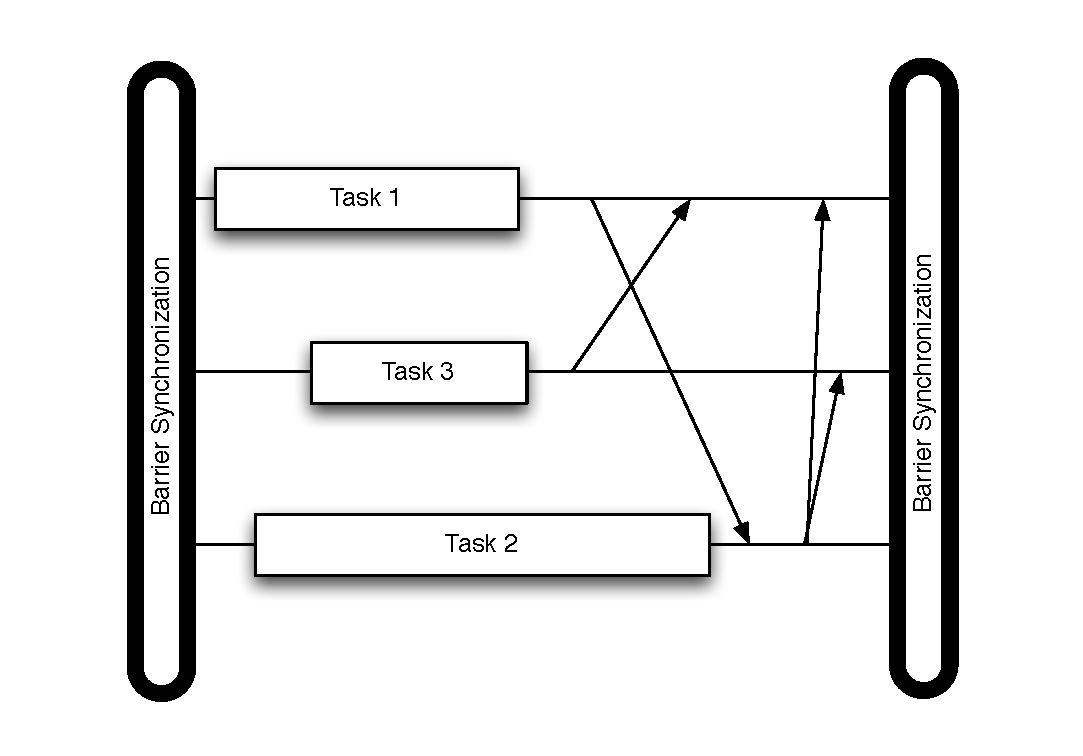
\includegraphics[width=0.5\linewidth]{img/BSP}
		%\vspace{-0.4cm}
		\caption{Un superstep dans le modèle BSP}\label{fig:Superstep}
\end{figure}

Une première implémentation du paradigme FIIT a vu le jour avec la plate-forme CONFIIT (Computation Over Network for FIIT) \cite{FKF03,Flauzac10}. CONFIIT a été développé en tant que middleware pour le calcul distribué, en s'appuyant sur un anneau logique (overlay) géré par le middleware et des échanges XML-RPC entre les n{\oe}uds. À la suite de sa version initiale, CONFIIT a été fortement modifié entre 2004 et 2006, avec l'addition de différents modes de calcul (distribué, centralisé), isolation (\textit{sandboxing}), observateurs extérieurs, etc. Ce développement a été fait notamment dans le cadre d'un projet supporté par l'agence ANVAR dans le but de créer une \textit{startup} dans le domaine du calcul distribué.
CONFIIT a été utilisé comme plate-forme de calcul pour plusieurs travaux, notamment lors de la résolution parallèle des instances L(2,23) et L(2,24) du problème de Langford \cite{JK04}.

Lors du démarrage du projet STIC-AmSud PER-MARE, nous avons voulu utiliser CONFIIT comme plate-forme pour l'exécution d'applications \textit{MapReduce}, mais nous avons rencontré plusieurs difficultés qui n'ont pas permis l'utilisation de CONFIIT pour la suite du projet. En effet, nous avons trouvé une faille dans la conception de l'anneau logique qui empêchait l'utilisation de CONFIIT pour les applications de type \textit{big data} : l'anneau était utilisé autant pour le passage des messages de service que pour la diffusion des données associées aux tâches. La transmission de masses de données plus importantes que quelques kilo-octets (ce qui était le cas avec Langford) occasionnait la congestion de l'anneau logique et empêchait la synchronisation des n{\oe}uds, causant ainsi leur déconnexion.

Après plusieurs tentatives, nous avons pris la décision de développer une nouvelle plate-forme, plus à jour et disposant de ressources capables de supporter aussi les applications de type \textit{big data}. Cette nouvelle implémentation, appelée CloudFIT, sera décrite dans les sections suivantes. 


\subsection{Spécification des besoins}

La décision d'implémenter une nouvelle plate-forme capable de supporter le paradigme FIIT (et ses variantes) dans un univers d'applications allant du calcul combinatoire au \textit{big data} a été suivie d'une liste d'exigences visant la généricité et la maintenance de la plate-forme :

\begin{description}
	\item [R1] CloudFIT doit être indépendant de l'overlay P2P. Ce choix rend possible le test de différents overlays P2P, afin de mieux s'adapter aux environnements et besoins des applications ;
	\item [R2] CloudFIT doit être modulable afin de supporter la composition et l'ajout de nouveaux modules, grâce à des interfaces et services bien définis. De plus, ceci doit permettre à l'utilisateur de composer "sa" pile logicielle sans avoir à modifier le code source, par exemple grâce à un fichier de configuration externe ;
	\item [R3] CloudFIT doit supporter le déploiement d'applications à la volée. Un utilisateur doit pouvoir soumettre ses propres classes applicatives à CloudFIT, qui les intégrera à la file d'exécution et les déploiera aux différents n{\oe}uds du réseau.
\end{description} 


L'objectif [R1] vient directement de l'expérience avec CONFIIT, où une dépendance trop forte par rapport au middleware P2P pourrait gêner l'évolution de la plate-forme. Comme les réseaux pervasifs présentent des grandes variations de performance et capacité, les couches les plus proches du réseau doivent pouvoir s'adapter à ces contraintes, comme par exemple l'impossibilité d'effectuer des diffusions, la présence de proxies et de passerelles NAT, voir même le support à des communications par mémoire partagée si l'environnement le supporte. Le respect à cet objectif a été très utile car l'overlay P2P initialement retenu (FreePastry\footnote{\url{http://www.freepastry.org/}}) s'est plus tard révélé peu performant et on a pu facilement migrer vers un nouvel overlay, TomP2P\footnote{\url{http://tomp2p.net}}. 

La règle [R2] est autant une prérogative visant l'évolution et la maintenance de la plate-forme qu'une manière de rendre plus simple l'expérimentation avec CloudFIT. De plus, le fait de reposer sur des interfaces permet une moindre dépendance entre les modules, demandant peu ou aucune modification de code en cas de remplacement d'un composant. 

Finalement, l'exigence [R3] garantit la scalabilité de la solution. En effet, il serait inconcevable d'avoir à distribuer l'application aux n{\oe}uds de calcul avant de lancer une application, comme c'était le cas avec CONFIIT. C'est bien le rôle de la plate-forme d'effectuer ce déploiement et d'assurer le lancement des applications selon des appels bien définis dans l'interface applicative. 

\subsection{Architecture}

L'architecture de CloudFIT a été conçue selon les objectifs cités précédemment. Afin de renforcer la modularité de la plate-forme, nous l'avons conçue sous la forme d'une pile logicielle, inspirée des modèles réseau TCP/IP et OSI. Ainsi, nous avons défini quatre couches représentant les différentes fonctionnalités de la plate-forme : \textbf{Network}, \textbf{Protocol}, \textbf{Service} et \textbf{Application}.

\begin{figure}
	\centering
		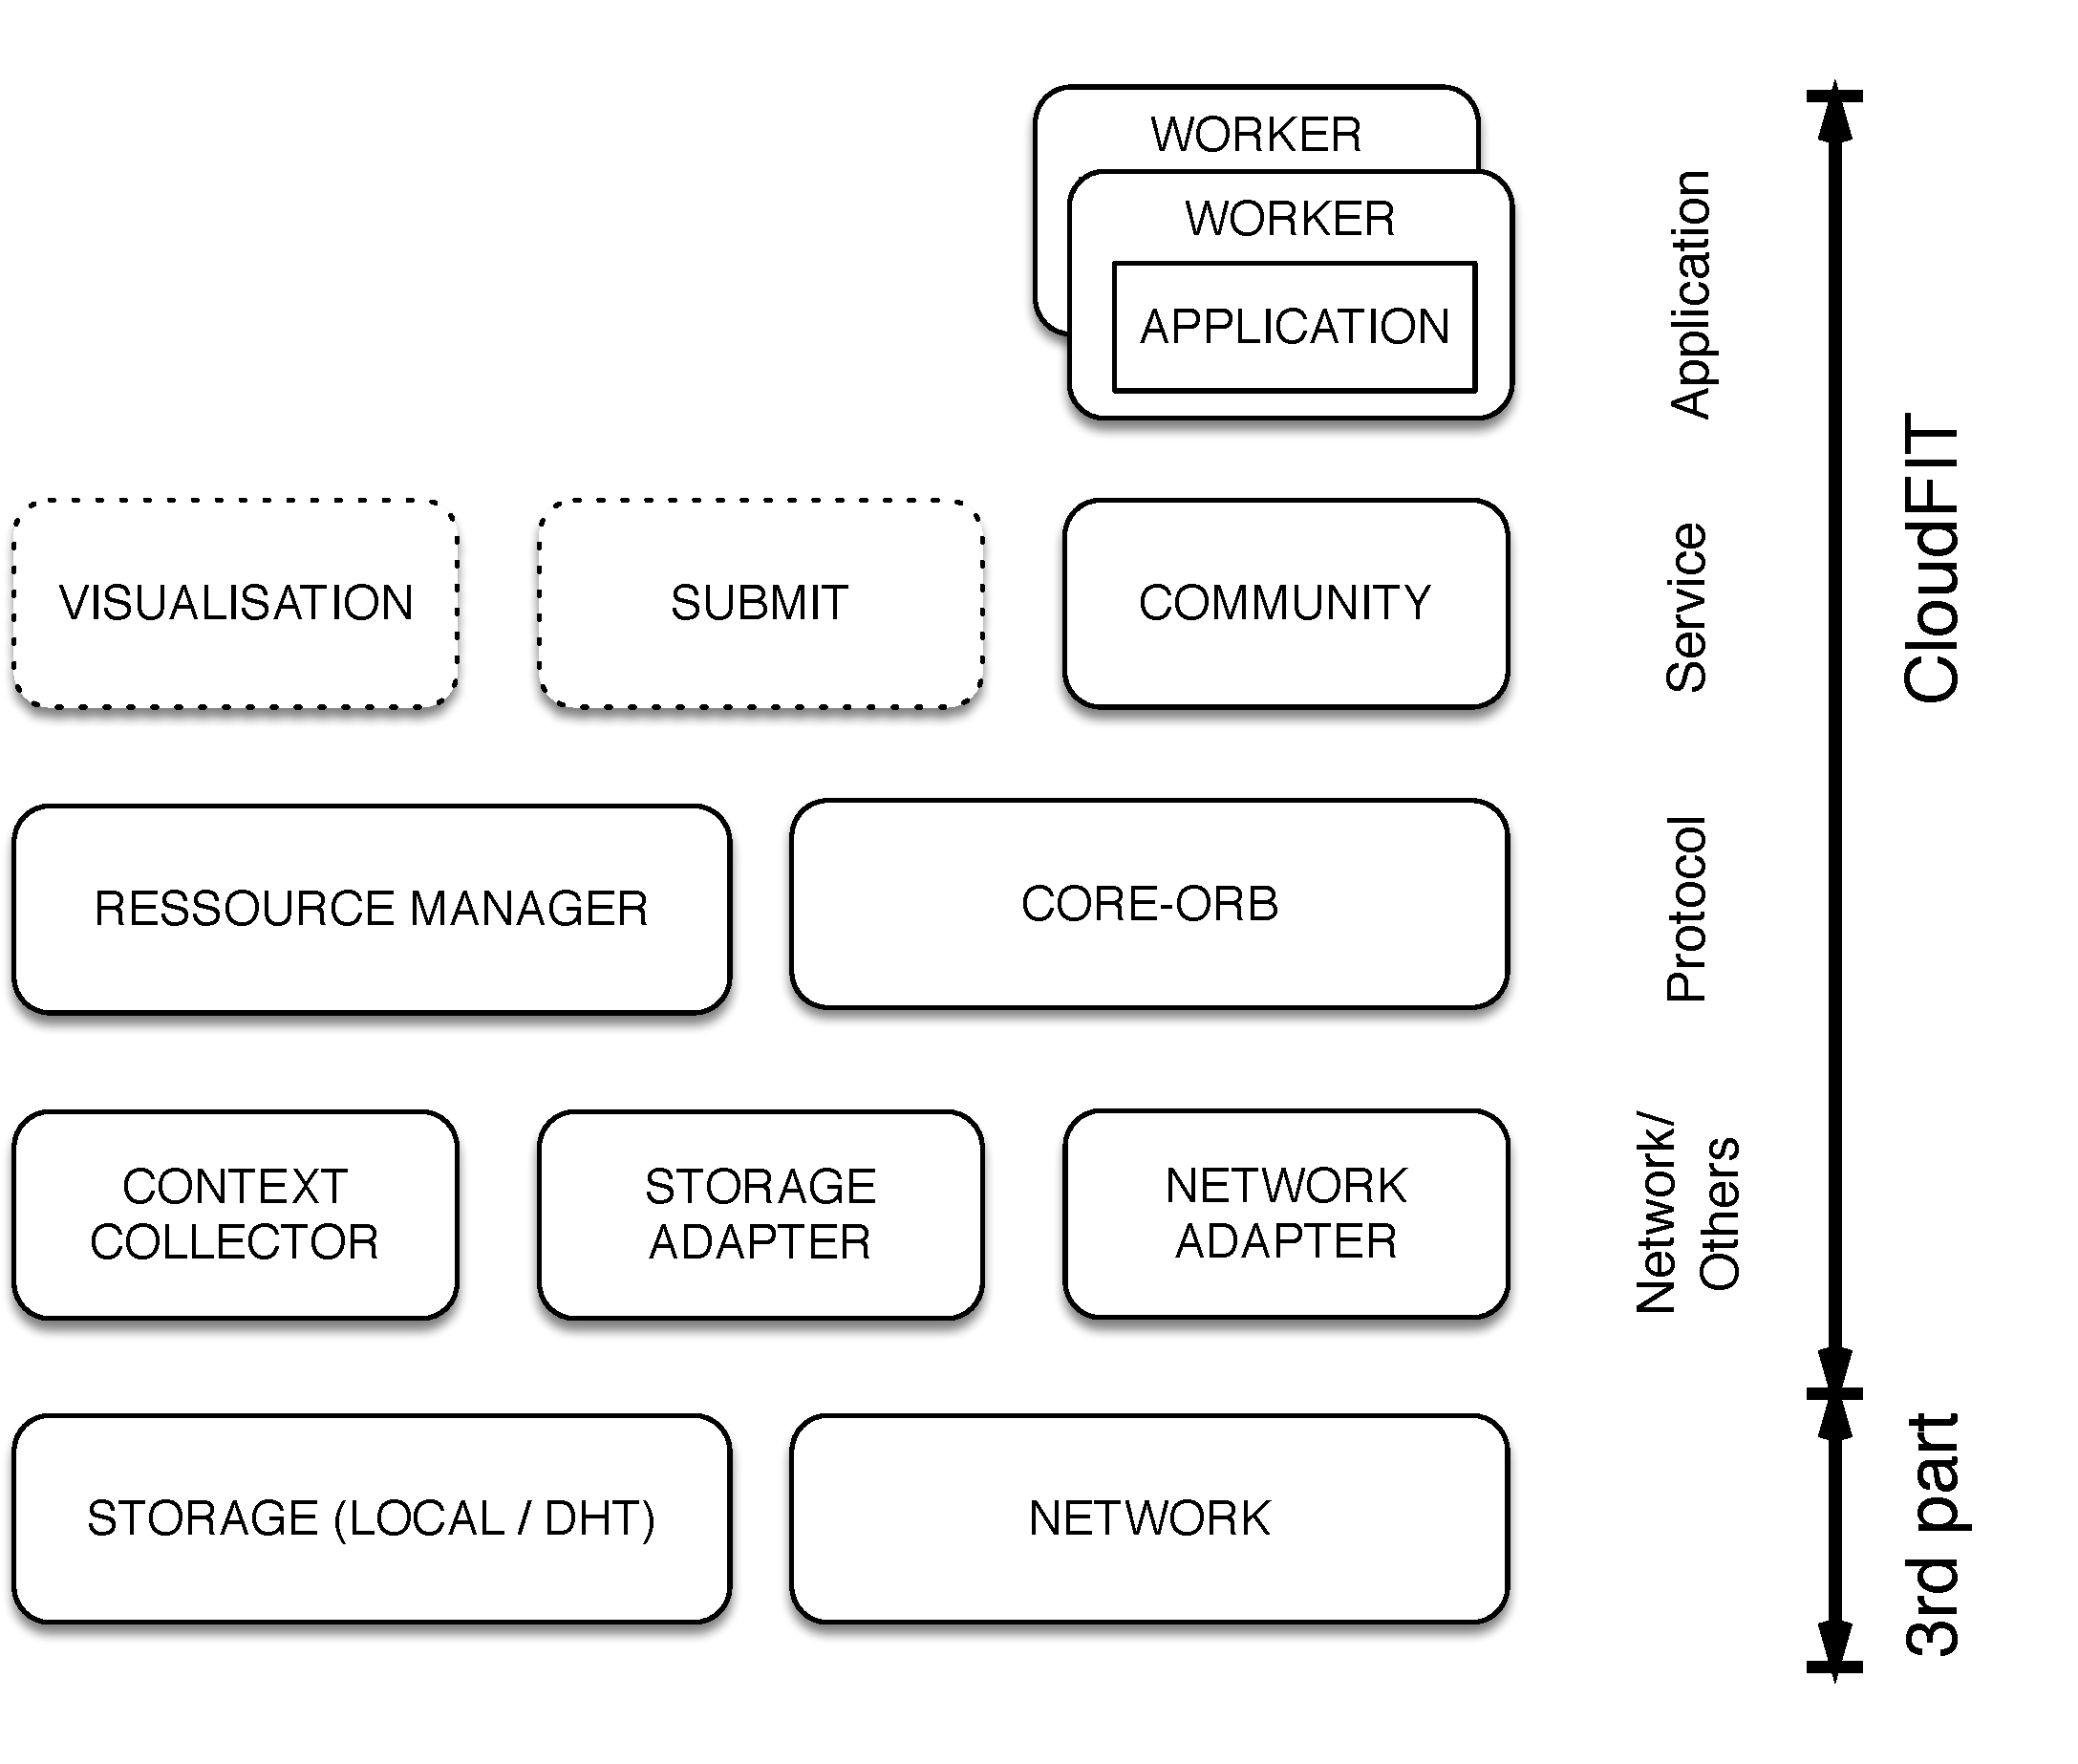
\includegraphics[width=0.65\linewidth]{img/CloudFITstack}
		\caption{Représentation simplifiée de la pile logicielle CloudFIT}\label{fig:cloudFitStack}
\end{figure}

Malgré son nom, la couche \textbf{Network} est responsable pour toute interaction avec les systèmes tiers sur lesquels CloudFIT s'appuie (overlay P2P, système  d'exploitation, systèmes de stockage). Par exemple, la classe \texttt{Network Adapter} exécute les opérations élémentaires d'encapsulation et décapsulation des messages, grâce à des primitives conçues selon les capacités des overlays P2P subjacents (\textit{send}, \textit{sendAll}, \textit{receive}, etc.). Le même principe s'applique à la classe \texttt{Storage Adapter}, où des primitives comme \textit{read}, \textit{write}, \textit{delete}, \textit{lookup} font l'interface avec les différentes solutions de stockage possibles (fichiers locaux, DHTs, bases de données, stockage sur le cloud). On y trouve finalement le \texttt{Context Collector}, déjà présenté dans le chapitre précédent en Section \ref{sec:gestionnairecontexte} et qui a été intégré à CloudFIT aussi.

La couche \textbf{Protocol} est responsable notamment par la gestion des messages et les ressources de calcul. Ainsi, le module \texttt{Core-ORB} (nommé ainsi car son rôle est comparable à celui d'un \textit{Object Request Broker}) stocke les messages reçus de la couche Network et délivre ces messages aux services adéquats de la couche supérieure. Grâce à un mécanisme \textit{publish-subscriber}, différents services peuvent s'enregistrer auprès le \texttt{Core-ORB}, obtenant ainsi un identifiant unique utilisé pour la réception des messages mais aussi pour des éventuelles communications entre les services dans le même n{\oe}ud. 

Le \texttt{Ressource Manager}, de son côté, puise dans les informations extraites par le collecteur de contexte pour vérifier si les ressources présentes dans la machine sont compatibles avec les besoins des applications. Ces besoins sont des propriétés fonctionnelles (mémoire disponible, espace disque, etc.) renseignées par l'application lors de sa soumission. Le \texttt{Ressource Manager} est aussi responsable pour la gestion du pool de \texttt{Workers}, qui sont alloués aux applications selon les demandes faites par les ordonnanceurs de tâches. 

La couche \textbf{Service}  contient les services nécessaires à l'exécution des applications distribuées. À cette couche appartient notamment la classe \texttt{Community}, une abstraction d'un groupe de machines qui gère le déploiement des applications et la gestion des événements liés aux n{\oe}uds (entrée, sortie, retransmission de messages, etc.). Chaque communauté est associée à un \texttt{JobScheduler}, qui gère la file d'applications soumises (jobs) et choisit lesquelles peuvent être lancées sur la machine, en croisant les contraintes des applications et les informations du \texttt{RessourceManager}.  Il faut remarquer que plusieurs communautés peuvent coexister sur un n{\oe}ud et dans le réseau, permettant ainsi la création de sous-ensembles de n{\oe}uds et le déploiement d'applications selon différents critères.

 D'autres services de cette couche incluent des interfaces de soumission ou de visualisation des résultats. Ces services sont notamment utiles dans l'interaction avec des dispositifs IoT qui n'ont pas la possibilité d'exécuter une instance de CloudFIT, comme par exemple les micro-contrôleurs Arduino. Dans ce cas, il suffit d'offrir un accès à un n{\oe}ud CloudFIT grâce à une interface REST ou JSON, comme suggère la Figure \ref{fig:cloudFitStackIoT}. Ces interfaces peuvent être utilisées autant pour le simple stockage de données que pour le déclenchement d'applications.

\begin{figure}
	\centering
		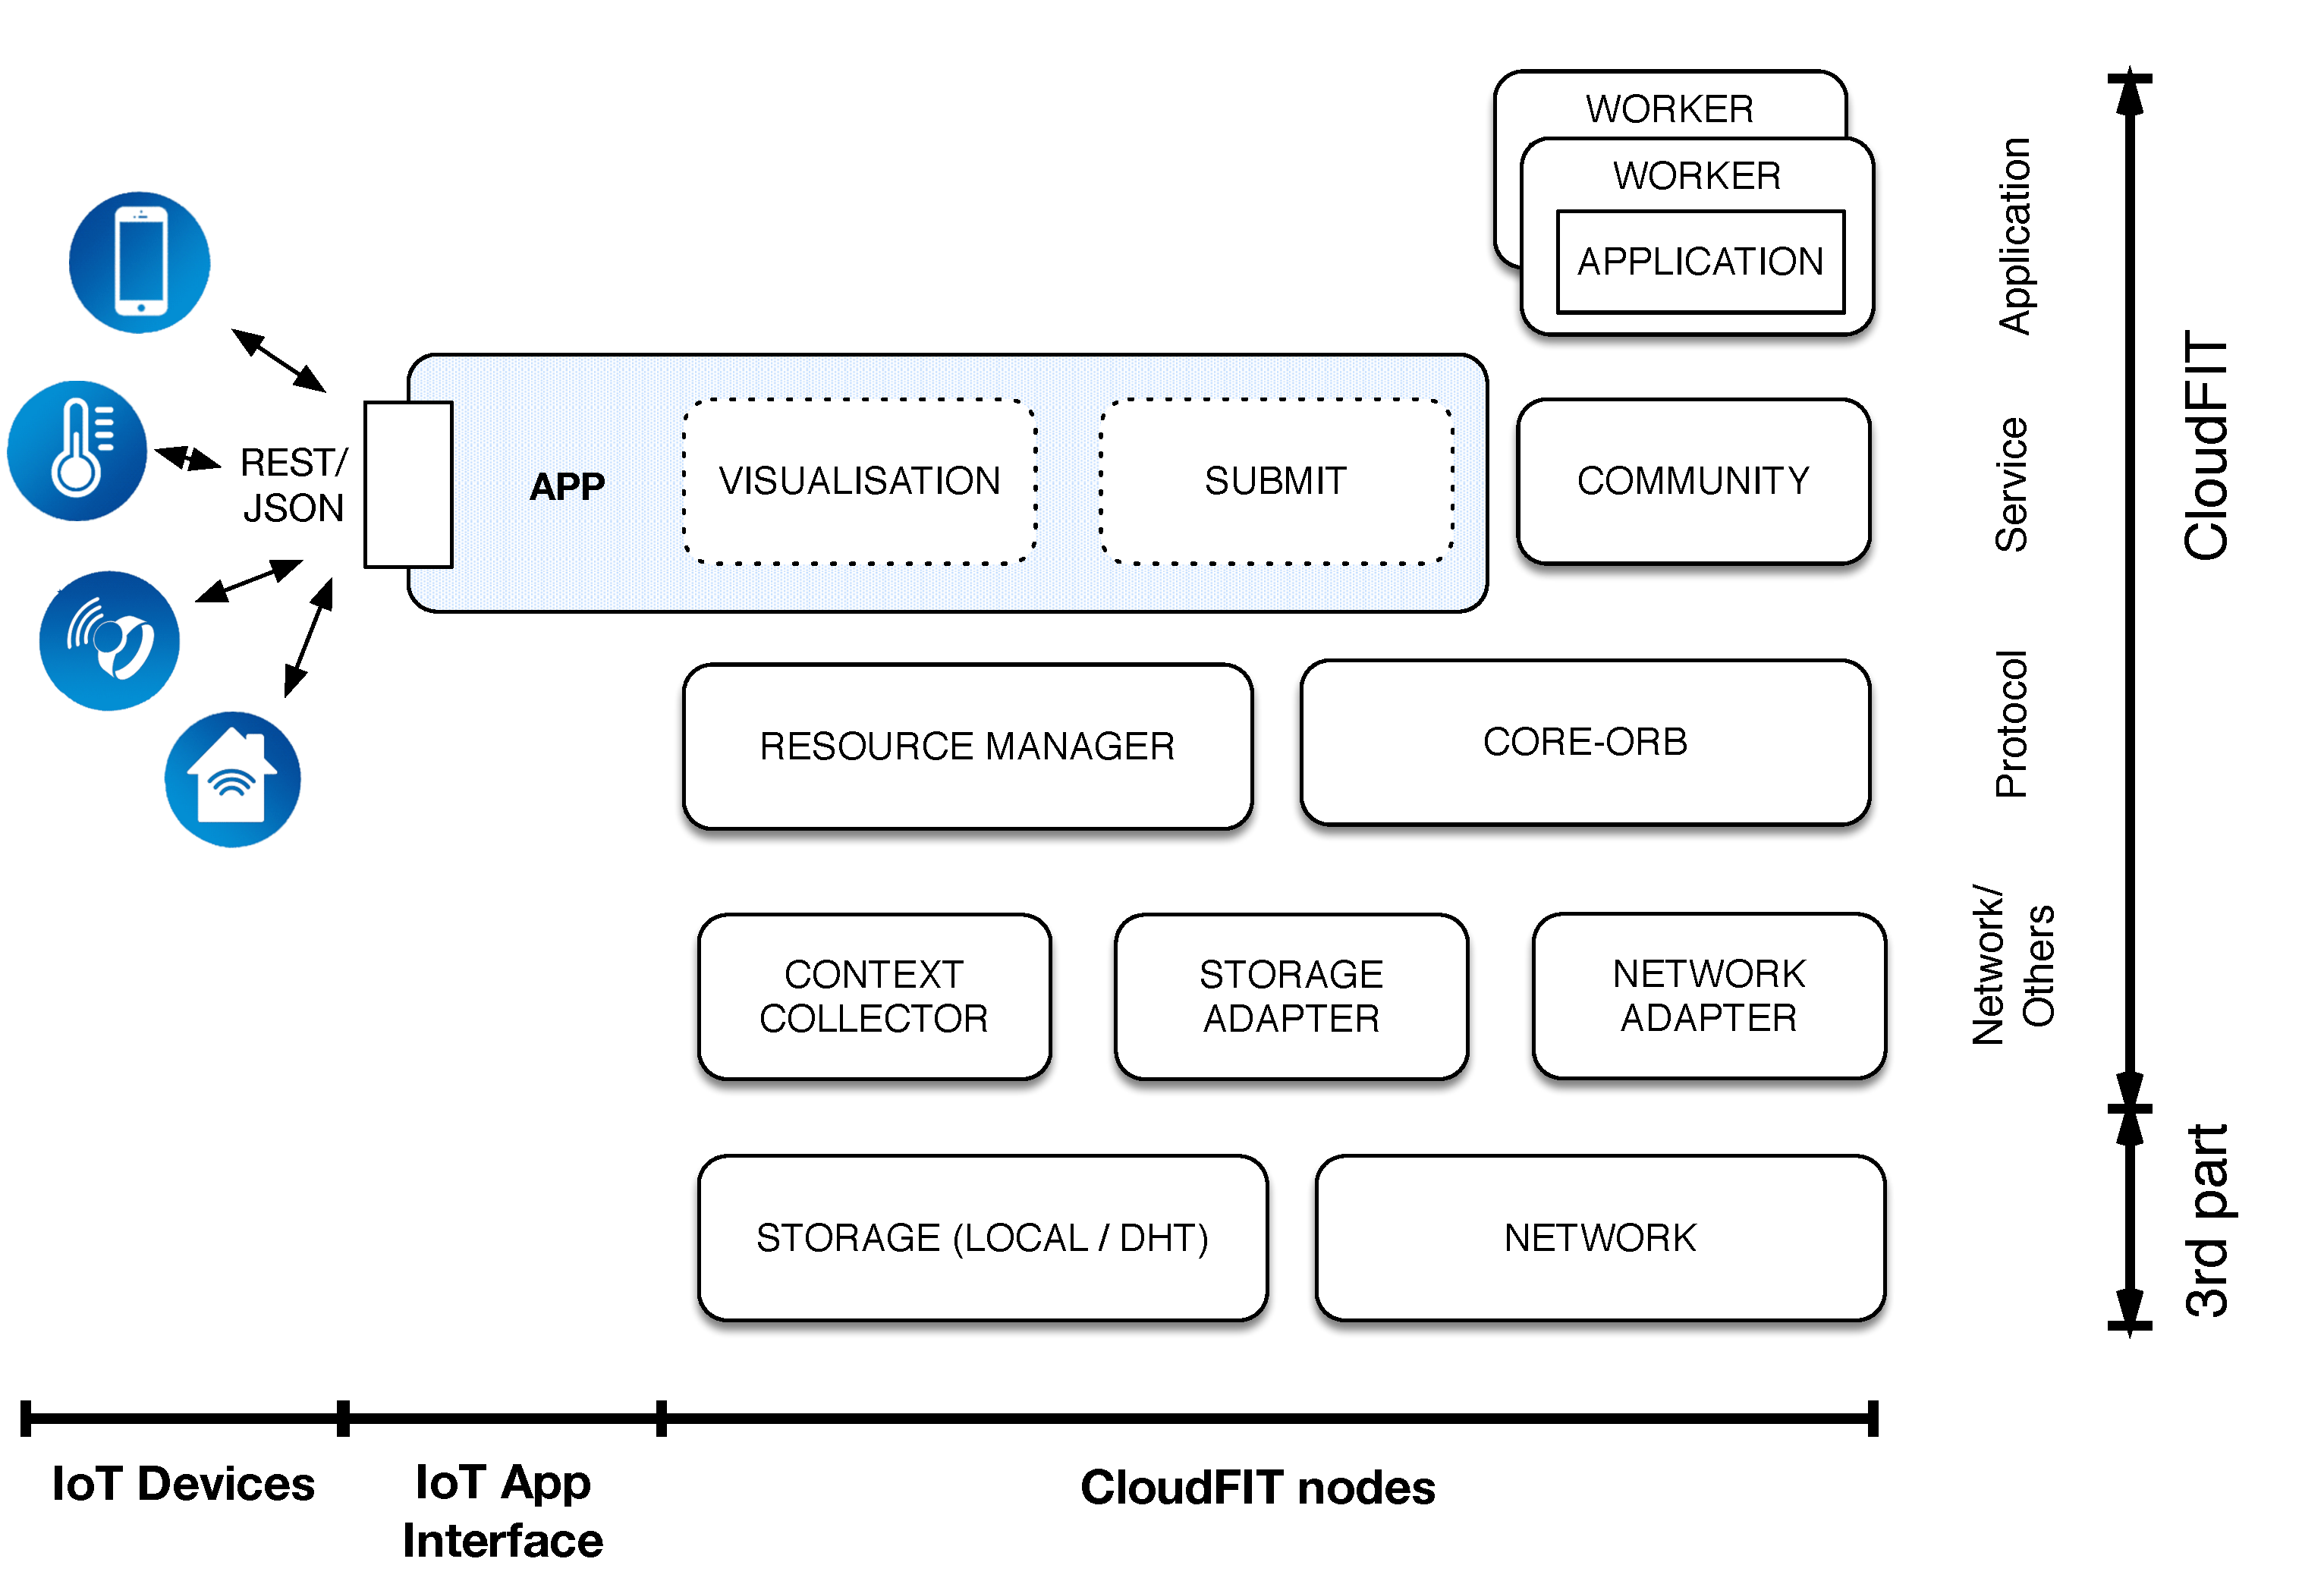
\includegraphics[width=0.65\linewidth]{img/CloudFITstack-IoT}
		\caption{Exemple d'interface IoT pour l'interaction avec CloudFIT}\label{fig:cloudFitStackIoT}
\end{figure}


Finalement, la couche \textbf{Application} contient les éléments nécessaires à l'exécution de l'application fournie par l'utilisateur. Cette couche spécifie l'interface applicative qui doit être implémentée par l'application utilisateur afin d'être exécutée par CloudFIT. L'interface applicative est assez simple et intuitive, suivant les principes du paradigme FIIT. Ainsi, le développeur n'a besoin que d'écrire les méthodes suivantes :
\begin{description}
	\item [numberOfBlocks()] méthode qui retourne le nombre de tâches à lancer. Cette méthode est appelée pendant la configuration du \texttt{TaskScheduler} ;
	\item [executeBlock(taskID, required{[]}) ] méthode qui démarre l'exécution proprement dite de la tâche, c'est le point d'accroche pour les \texttt{Workers}. Le \textit{taskID} permet à la tâche de personnaliser son exécution, et l'élément \textit{required[taskID]} indique les éventuelles dépendances de cette tâche. Ce paramètre est aussi utilisé par le \texttt{TaskScheduler} pour gérer l'ordre d'exécution afin de respecter les dépendances ;
	\item [finalizeApplication()] méthode optionnelle qui est exécutée par le \texttt{TaskScheduler} une fois que l'ensemble de tâches est terminé. Cette méthode permet l'agrégation des résultats, à l'instar d'une phase Reduce dans le paradigme \textit{MapReduce}.
\end{description}

On y trouve aussi la classe\texttt{ TaskScheduler}, un ordonnanceur associé à chaque job et responsable par la gestion des tâches et l'interaction avec le \texttt{RessourceManager} afin d'obtenir des \texttt{Workers} pour exécuter ces tâches. L'interaction entre le \texttt{TaskScheduler}, l'application et les autres éléments de la couche Service est présentée de manière simplifiée en Figure \ref{Figure:applayer}. 

\begin{figure}
	\centering
		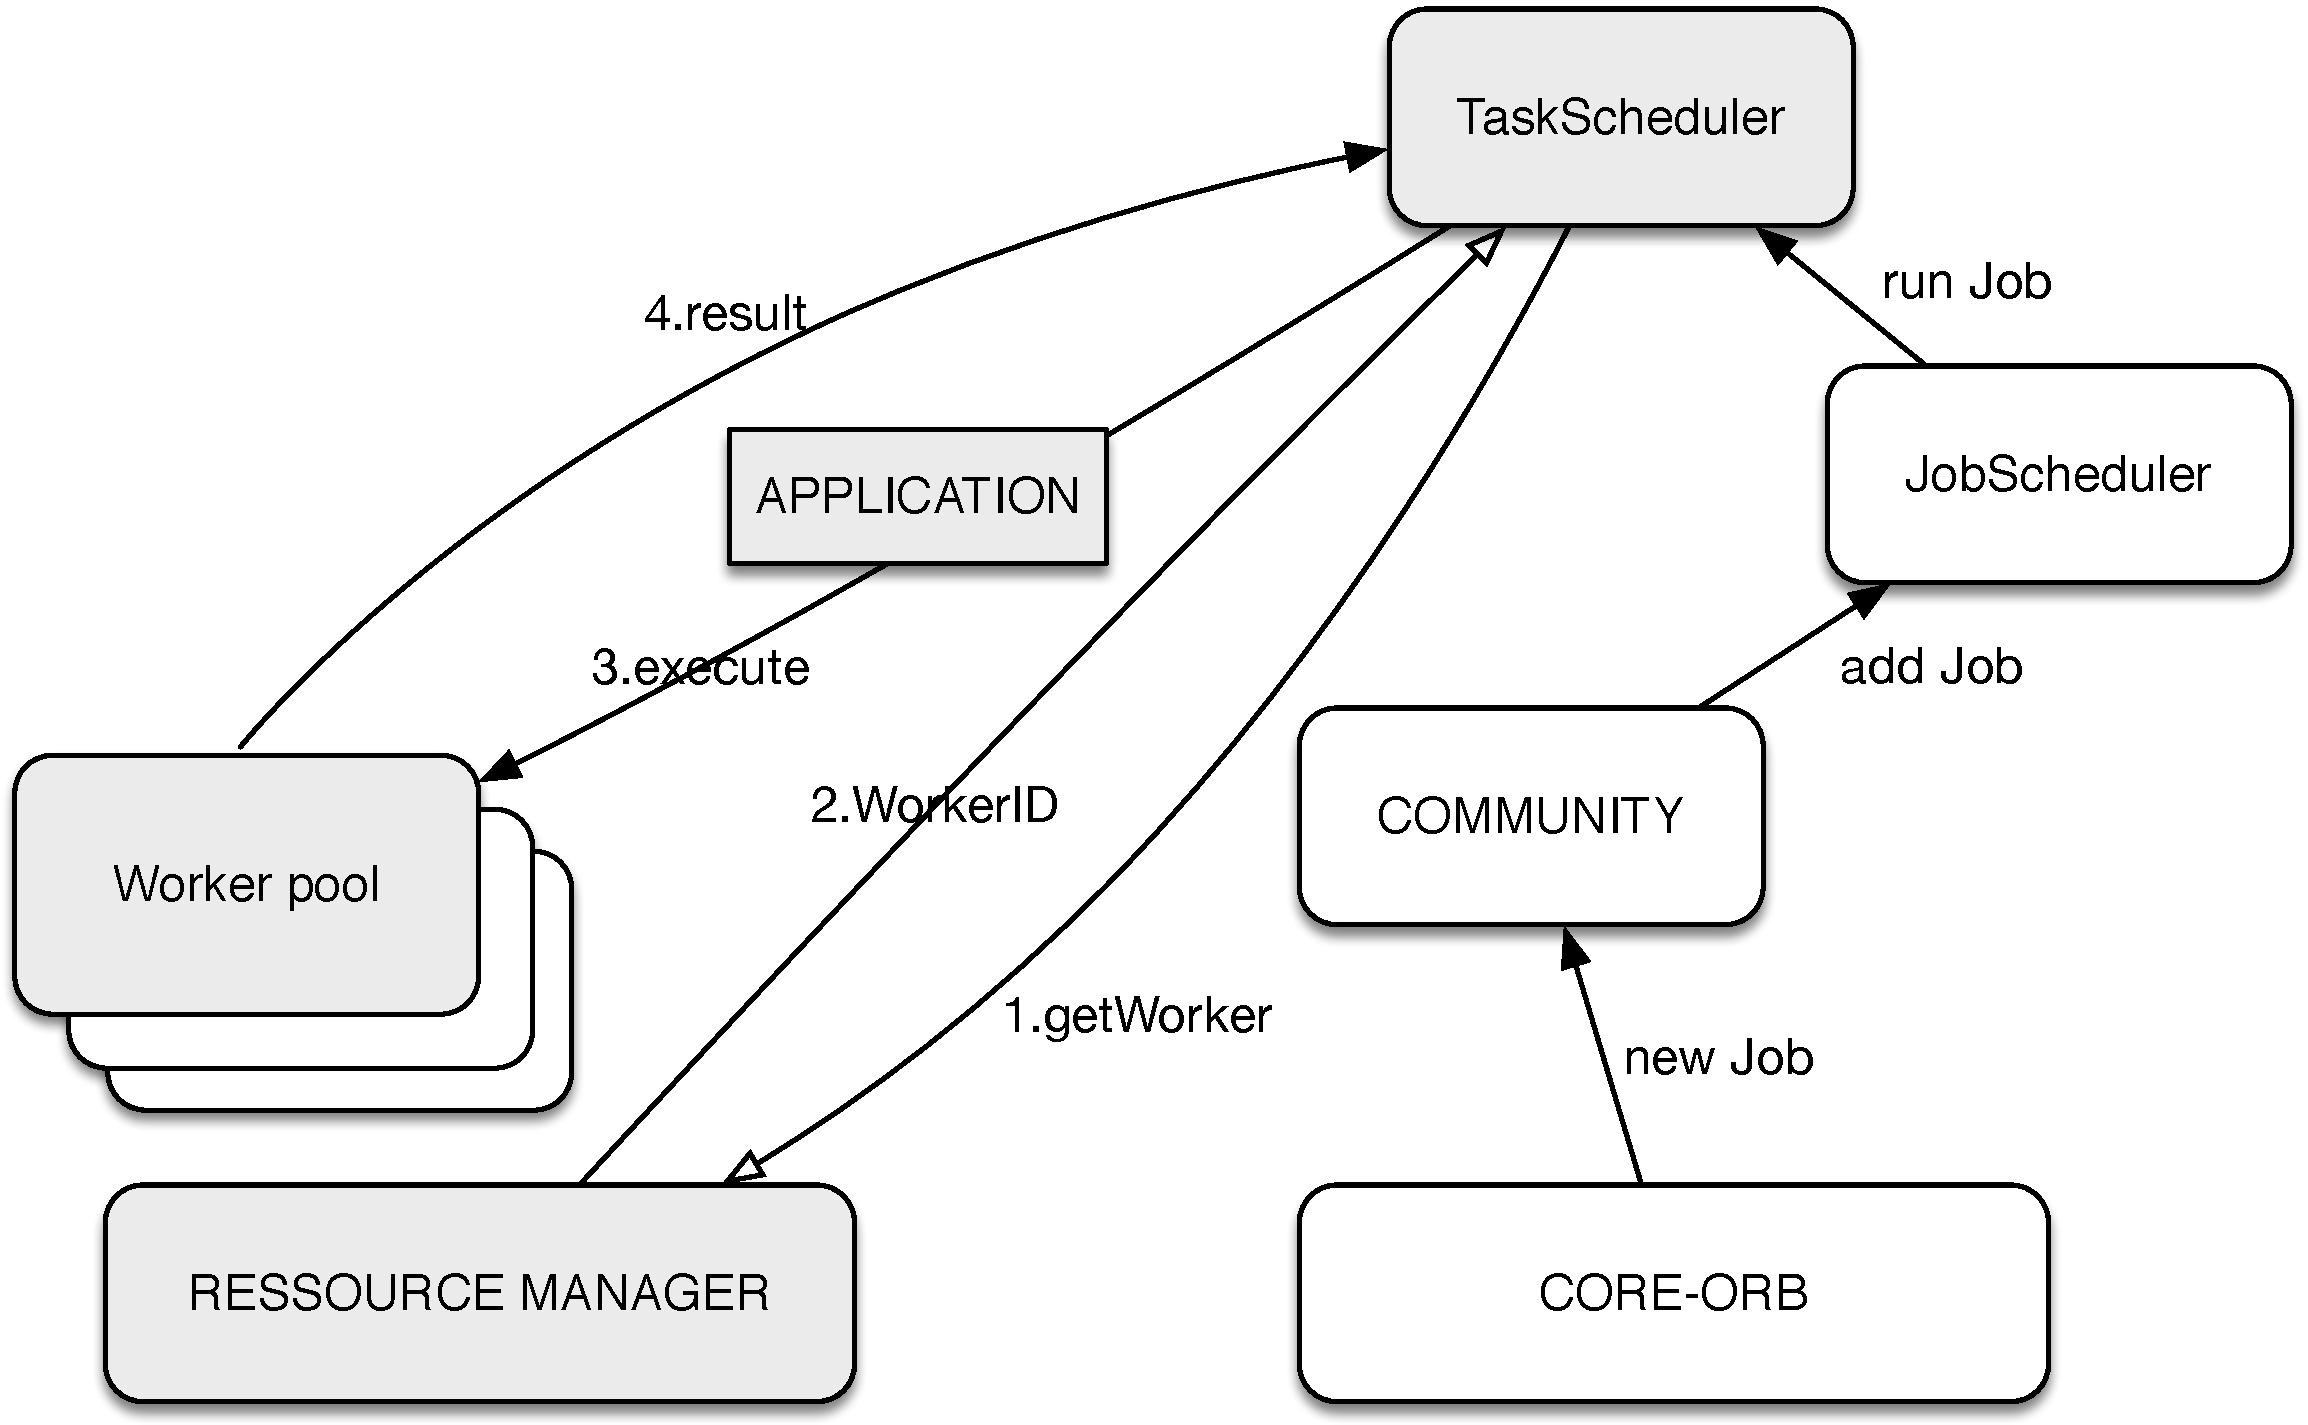
\includegraphics[width=0.65\linewidth]{img/CloudFITstack-app}
		\caption{Diagramme simplifié de l'interaction entre les éléments lors du lancement d'un job et de ses tâches}\label{Figure:applayer}
\end{figure}

Il faut noter que la classe \texttt{TaskScheduler} est extensible et personnalisable. Par défaut CloudFIT fournit un ordonnanceur simple, mais celui-ci peut être remplacé par des ordonnanceurs plus élaborés. L'ordonnanceur par défaut fait juste une redistribution aléatoire des tâches, une technique simple qui réduit le risque de travail en doublon entre les n{\oe}uds. Parmi les exemples d'ordonnanceurs plus élabores on peut citer ceux qui prennent en charge les dépendances entre les tâches (dans le cas d'une application DAG) ou qui utilisent des éléments de contexte comme par exemple la localisation d'un n{\oe}ud pour minimiser le temps d'accès aux données. 




\subsection{Communication\label{subsec:commCloudFIT}}

La section précédente illustrait la structuration et l'interaction des modules dans une machine. Cependant, une plate-forme de calcul distribué se doit de garantir les échanges entre les différents n{\oe}uds sur le réseau. Dans le cas de CloudFIT, le choix d'utiliser un overlay P2P tiers simplifie les opérations de découverte de pairs, la gestion du réseau (entrées, sorties), routage des messages, etc. Nous pouvons ainsi nous concentrer sur la communication intrinsèque à la plate-forme, comme par exemple le déploiement des applications, le suivi de la progression de l'exécution et la distribution/récupération des résultats. 

Tout démarre par la soumission d'un job, effectué directement par un n{\oe}ud déjà connecté au réseau ou grâce à une interface de soumission. Cette soumission contient le code applicatif, le nom de la Community cible, ainsi qu'une liste de propriétés nécessaires à la bonne exécution du job. Ce message est envoyé à travers le réseau, grâce aux mécanismes de diffusion de l'overlay P2P ou, le cas échéant, grâce à une diffusion de type \textit{best-effort}.

Comme spécifie l'objectif [R3], nous devons garantir qu'une application sera déployée par la plate-forme elle-même car il serait très contraignant pour l'utilisateur de placer l'application sur chaque n{\oe}ud. Afin de répondre à ce besoin, nous avons choisi d'utiliser le stockage DHT habituellement associé aux overlays P2P. En effet, le DHT offre à tous les n{\oe}uds de l'overlay un accès réseau à des objets et fichiers, du moment où ces n{\oe}uds connaissent la clé des ressources. Ainsi, la soumission d'un job comprend l'enregistrement d'un fichier \textit{jar} contenant le code applicatif et la clé DHT de cette ressource. Au moment du lancement du job, le \texttt{JobScheduler} récupère ce fichier et extrait ses classes, qui seront chargés grâce à un \textit{classloader}. 

Le stockage DHT peut aussi être utilisé pour la mise à disposition de données d'entrée pour les applications, comme par exemple dans le cas d'une application \textit{big data}. Ceci n'est pas obligatoire, vu que les applications ont aussi la possibilité d'obtenir les données via des ressources extérieurs (URLs, stockage cloud, bases de données).

Lorsqu'un job démarre sur une machine, son statut passe de \textit{NEW} à \textit{STARTED}. À ce moment le \texttt{TaskScheduler} associé à ce job est démarré, et les tâches peuvent être lancées. Celles-ci ont 5 états possibles : \textit{NEW}, \textit{STARTED}, \textit{STARTED\_DISTANT}, \textit{COMPLETED} et \textit{DISTANT}. 

Lorsqu'une tâche est lancée, un message est envoyé aux n{\oe}uds de la \texttt{Community} indiquant le ID du job et de la tâche. Ceci permet aux \texttt{TaskScheduler} des autres n{\oe}uds de savoir cette tâche est traitée par une autre machine et ainsi réduire le travail en doublon : ces tâches "distantes" sont marquées comme \textit{STARTED\_DISTANT} et sont placées à la fin de la file d'exécution. Une tâche marquée ainsi ne sera exécutée que lorsque toutes les tâches \textit{NEW} ont été épuisées et, bien sûr, si aucun message n'est venu indiquer que la tâche a été complétée. En effet, le \texttt{TaskScheduler} envoie un deuxième message à la fin de l'exécution d'une tâche, indiquant le changement de son statut à \textit{COMPLETED} et aussi indiquant le résultat de son calcul (ou bien les coordonnées pour retrouver ce résultat, si stockés dans la DHT ou dans une ressource externe).

Si un n{\oe}ud finit l'exécution de toutes ses tâches \textit{NEW}, il peut démarrer l'exécution de tâches spéculatives parmi celles marquées \textit{STARTED\_DISTANT}. Ce mécanisme garantit la terminaison de toutes les tâches (si le n{\oe}ud original est défaillant) et permet même d'accélérer la terminaison du calcul si le n{\oe}ud original est trop lent.

En plus de mettre à jour les autres n{\oe}uds, ces échanges de messages ont aussi le rôle de mettre au courant un nouveau n{\oe}ud qui rejoint le réseau. En voyant passer des messages de type "task completed", les n{\oe}uds peuvent demander à un voisin de les transmettre le message avec la description du job. Son \texttt{TaskManager} va donc procéder à la récupération des tâches \textit{DISTANT} grâce à des requêtes spécifiques. Ce mécanisme permet ainsi de garantir l'intégration des n{\oe}uds dans un environnement volatile et d'assurer la pérennité des résultats. En effet, il suffit qu'une machine subsiste dans le réseau pour que les résultats restent accessibles.

À la fin de l'exécution de toutes les tâches, les \texttt{TaskManager} récupèrent l'ensemble des résultats locaux ou distants et le statut du job devient \textit{COMPLETED}. Ce job reste à la disposition de toute application ou n{\oe}ud qui souhaite récupérer ses résultats.


\section{Calcul Multi-échelle et le \textit{Fog Computing}}

Comme indiqué précédemment, la plupart des travaux sur le \textit{edge/fog computing} ont la tendance à faire une distinction entre l'utilisateur final (ou les périphériques finaux) et les dispositifs qui se trouvent à la frontière de l'Internet/\textit{cloud}. Dans de telles approches, les appareils IoT sont des simples clients des services déployés dans un voisinage proche, ce qui est d'une certaine manière contraire aux principes du \textit{fog computing}, où tous les dispositifs peuvent contribuer au calcul des tâches selon leurs propres capacités et ressources disponibles. 

Cependant, les réseaux P2P les plus connus organisent les n{\oe}uds indistinctement de leur emplacement réel, ce qui empêche l'établissement de services de proximité à faible latence. Pour contourner ces inconvénients, nous considérons que le réseau P2P de CloudFIT doit être enrichi par l'utilisation du concept du calcul multi-échelle \cite{Rottenberg2012,Rottenberg2014}  associé à des techniques de \textit{clustering}. En effet, le regroupement des ressources sous la forme de \textit{clusters} est une manière efficace pour organiser les couches de calcul multi-échelle et ainsi fournir une base de coordination pour le déploiement efficace des services.

\subsection{Clustering}

Plusieurs approches de clustering sont proposées dans la littérature \cite{Johnen2011} et utilisées, par exemple, pour  le routage des informations dans les réseaux de capteur sans fil. La plupart des algorithmes de clustering utilisent des paramètres simples comme la densité du réseau environnant, choisissant un \textit{cluster-head} en fonction de leurs identités uniques (ID). Malheureusement, ces métriques sont insuffisantes pour assurer le clustering dans un scénario hétérogène, vu qu'elles ne permettent pas d'exprimer les besoins du calcul multi-échelle. 

Dans notre cas, nous devons permettre le regroupement des n{\oe}uds selon différentes stratégies de manière à co-localiser les données et les ressources nécessaires pour les services de proximité mais aussi faire des ponts pour relier les dispositifs proches et ceux plus éloignés, même jusqu'au cloud. Ainsi, afin de s'adapter à l'hétérogénéité des environnements pervasifs et l'IoT, les métriques de clustering doivent inclure des informations de contexte telles que la proximité, les capacités informatiques et de stockage des appareils, la fiabilité et même le niveau d'autorisation/confiance des n{\oe}uds collaborateurs.
 
Dans le cas de CloudFIT, ce clustering peut être mis en {\oe}uvre grâce aux \textit{communautés}, en créant des sous-ensembles de n{\oe}uds qui peuvent être adressés séparément et donc utilisés pour répartir/cloisonner les opérations. Bien entendu, un n{\oe}ud peut appartenir à plusieurs communautés, permettant à des données et des tâches de circuler entre les différentes couches multi-échelle, comme illustrée en Figure \ref{fig:antennes}. Cette organisation à plusieurs niveaux en fonction du contexte des ressources disponibles permettrait de mieux coordonner la communication entre ces ressources et d'ainsi mieux gérer la variabilité d'échelle de ces environnements. 

 
 \begin{figure}[!ht]
 	%\renewcommand{\figurename}{Figura}
 	\centering
 	%\vspace{-0.3cm}
 	\includegraphics[width=0.6\linewidth]{img/antennes2.pdf}
 	%\vspace{-0.2cm}
 	\caption{Exemple de communautés interconnectées dans une plate-forme multi-échelle}
 	\label{fig:antennes}
 	%\vspace{-0.5cm}
 \end{figure}

\subsection{Optimisations pour le \textit{big data}}
%
Dans le cadre du traitement de données issus des dispositifs de l'IoT, un autre facteur à prendre en compte est celui de la performance liée à l'accès et à la gestion des données. En effet, la plupart des opérations impliquent la collecte, la transformation et l'analyse des données, et les plates-formes telles que Apache Hadoop se sont illustrées par leur capacité d'optimiser l'accès aux données en plaçant les tâches préférentiellement là où les données sont présentes (grâce au concept de la \textit{data locality}). 

Dans le passé \cite{Steffenel2015Roma} nous avons déjà mené des expérimentations avec CloudFIT démontrant que des performances similaires ou supérieures à celles de Apache Hadoop pourraient être atteintes avec un système P2P, comme illustré en Figure \ref{fig:Hadoop}. Bien que ces résultats aient été positifs, nous avons observé deux points qui pourraient être encore améliorés : la surcharge de gestion des données sur un n{\oe}ud et la prise en charge de la \textit{data locality}. 

\begin{figure}[!ht]
	%\renewcommand{\figurename}{Figura}
	\centering
	%\vspace{-0.3cm}
	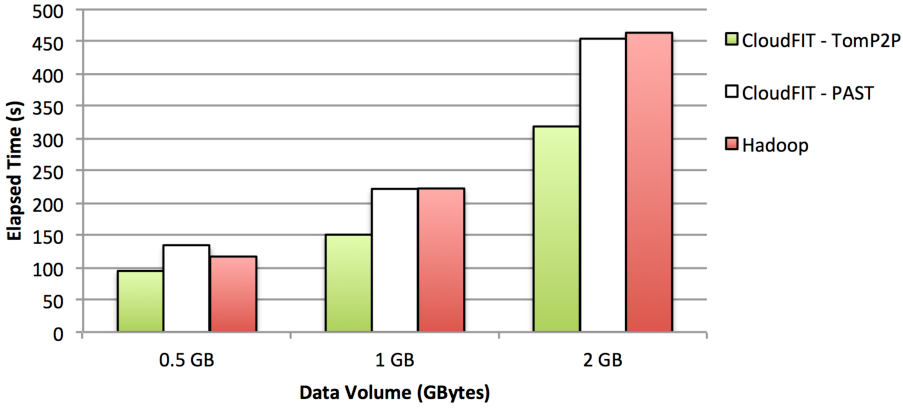
\includegraphics[width=0.65\linewidth]{img/CloudFIT-mesures.pdf}
	%\vspace{-0.2cm}
	\caption{Comparaison des temps d'exécution de WordCount avec CloudFIT et Hadoop}
	\label{fig:Hadoop}
	%\vspace{-0.2cm}
\end{figure}

Dans le premier cas, nous avons constaté un fort écart de performances d'accès aux données lorsque nous déployons CloudFIT  dans un environnement hétérogène. Ces écarts de performance sont en effet une combinaison de la vitesse d'accès aux données et de la surcharge de gestion des systèmes de stockage (voir aussi les limitations physiques de stockage), et affectent notamment les dispositifs de faible capacité. Ainsi, par exemple, un Raspberry Pi est fortement pénalisé par la vitesse et la capacité de stockage de sa carte SD, malgré une capacité de calcul suffisante (notamment en utilisant tous ses c{\oe}urs de calcul).  

Afin de contourner cette limitation, nous avons modifié la couche de stockage de manière à ce que les n{\oe}uds puissent choisir d'agir seulement en tant que clients distants. Ces n{\oe}uds peuvent donc interroger le service de stockage DHT via le réseau mais ils ne sont plus obligés à gérer le stockage, réduisant leur surcharge et aussi leur utilisation du disque.

Pour ce qui est de la prise en charge de la \textit{data-locality}, cela est un problème plus général qui affecte la plupart des architectures de stockage P2P. En effet, les API de stockage P2P sont souvent basés sur les tables de hachage distribuées (DHT). Ces DHTs sont conçues de manière à répartir les données sur le réseau et les répliquer lorsque cela est possible, notamment afin d'éviter la perte de données en cas de désabonnement (\textit{churn}). Un inconvénient de cette procédure est qu'on observe une perte d'information concernant la localisation des données \cite{Wu2005}, rendant difficile l'optimisation des transferts réseau. Nous avons donc développé deux mécanismes distincts visant à contourner cette limitation. 

La première approche que nous avons développée peut facilement être mise à l'{\oe}uvre si on un accès à la bibliothèque DHT. Cette stratégie consiste à instruire l'ordonnanceur de tâches (\textit{TaskScheduler}) à vérifier préalablement quelles tâches seraient favorisées par la présence des données dans son cache DHT local. Même si c'est une opération de bas niveau, la plupart des DHT P2P offrent la possibilité d'effectuer un \textit{lookup} pour savoir si la ressource requise se trouve déjà dans le cache local ou s'il faut la chercher sur le réseau. En donnant la priorité aux tâches qui peuvent travailler avec des données locales, on peut espérer augmenter la performance globale de l'exécution.

Toutefois, il n'est pas toujours possible d'avoir des données en local dans un overlay P2P. En effet, dans une DHT les n{\oe}uds responsables par le stockage et indexation des ressources sont définis par la clé de hachage de la ressource. La Figure \ref{fig:pastry} illustre le cas du routage d'un message dans l'overlay Pastry \cite{Pastry01, Castro2002}, mais le même exemple peut être utilisé pour la localisation des ressources dans la DHT PAST \cite{Rowstron2001b} car dans ce système les clés des ressources et les clés des n{\oe}uds se superposent. Finalement, même avec de la réplication, il y a le risque que dans un grand réseau les ressources ne se trouvent sur aucun des n{\oe}uds de calcul. Ceci nous amène à l'élaboration d'une stratégie pour renforcer la proximité des données, grâce à un calcul personnalisé de la clé de localisation des ressources. 


\begin{figure}[!ht]
	%\renewcommand{\figurename}{Figura}
	\centering
	%\vspace{-0.3cm}
	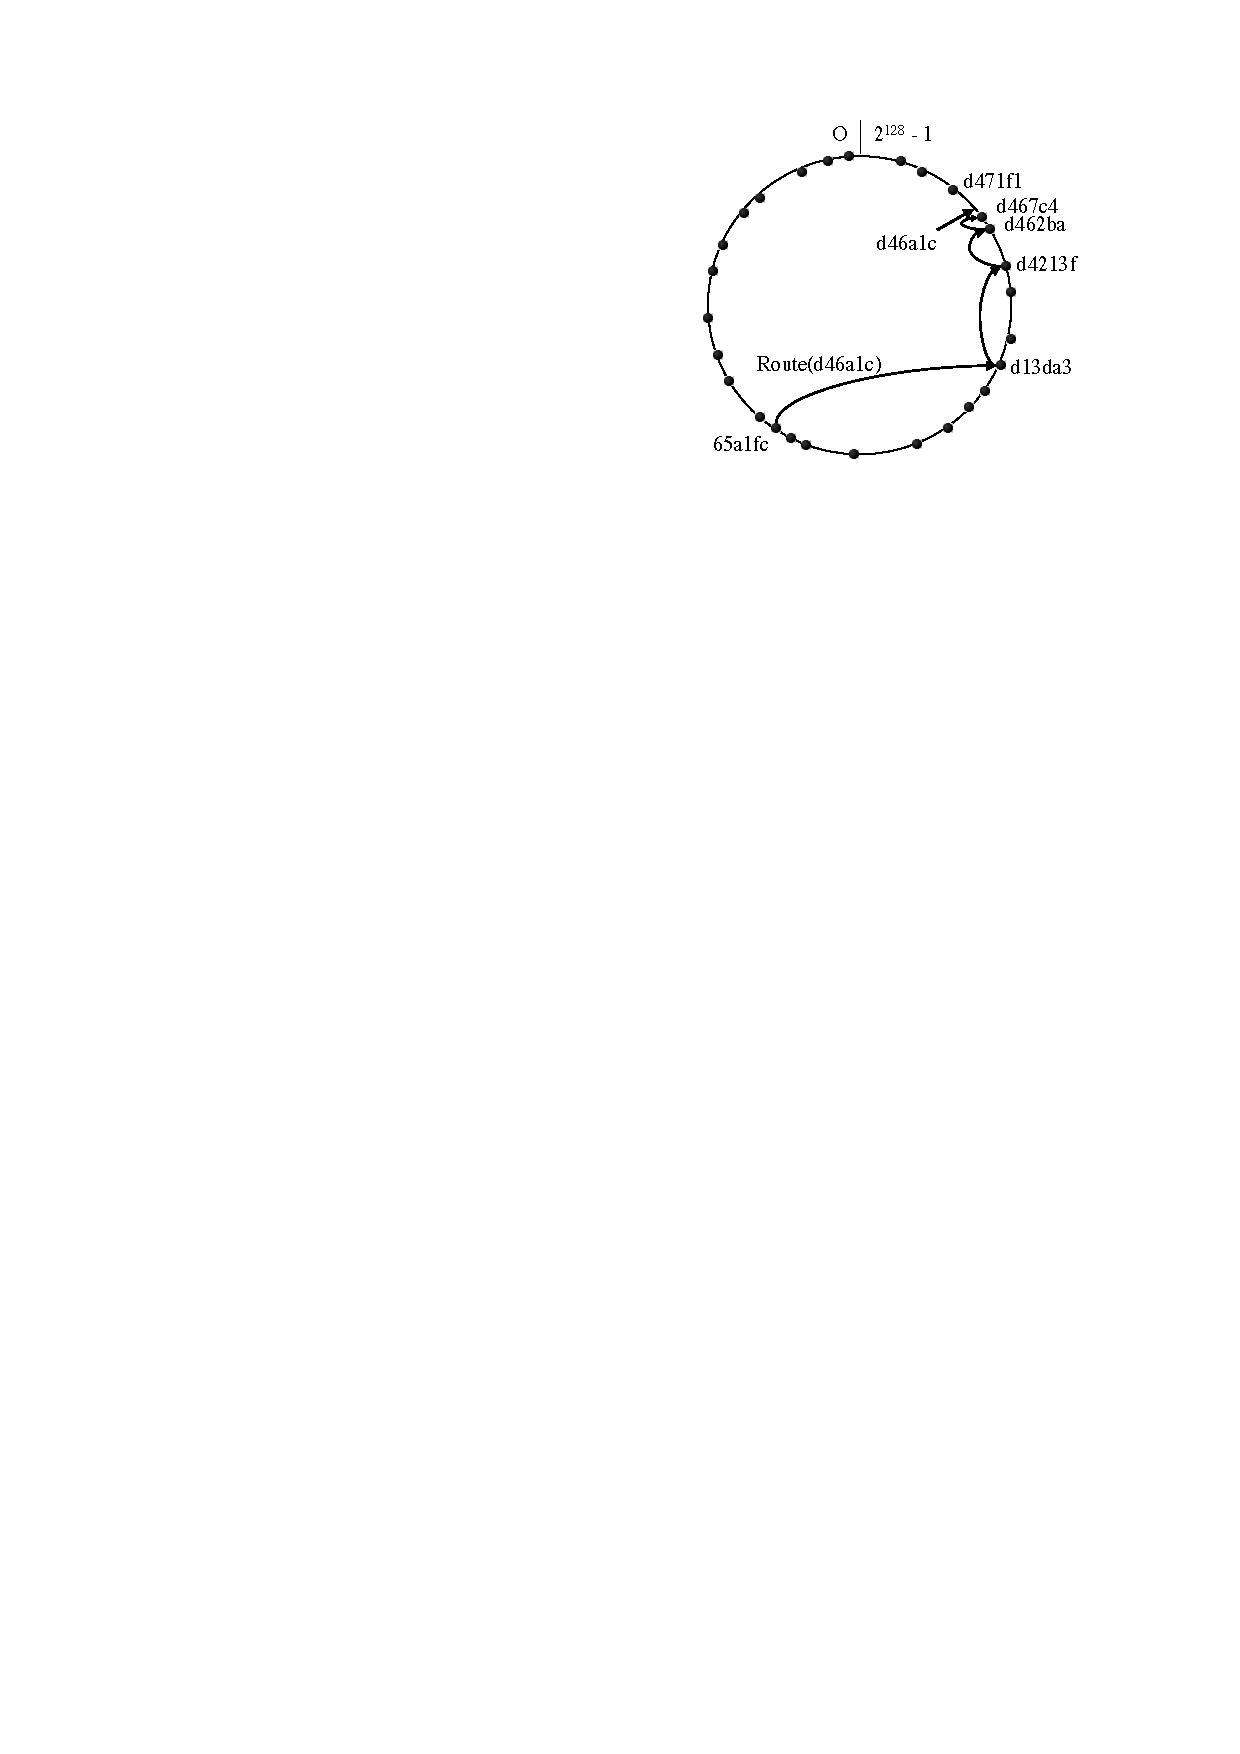
\includegraphics[width=0.4\linewidth]{img/AnneauPastry.pdf}
	%\vspace{-0.2cm}
	\caption{Exemple de routage d'un message dans l'overlay Pastry \cite{Castro2002}}
	\label{fig:pastry}
	%\vspace{-0.2cm}
\end{figure}


Cette technique a été élaborée sur la base des spécificités de la DHT de TomP2P, et donc ne peut pas être facilement généralisée. Contrairement à la plupart des systèmes de P2P qui ont seulement une clé de hachage, TomP2P identifie les ressources par quatre clés différentes $\{k_l,k_d,k_c,k_v\}$, selon la hiérarchie suivante : 
\begin{itemize}
	\item \textit{$k_l$} - clé de localisation, utilisée pour la localisation d'une ressource dans la DHT ;
	\item \textit{$k_d$} - clé de domaine, fonctionne comme une clé d'authentification, permet la séparation des données ;
	\item \textit{$k_c$} - clé de contenu, permet d'identifier une ressource. Par défaut celle-ci est identique à la clé de localisation ;
	\item \textit{$k_v$} - clé de version, permet la gestion de versions multiples d'une ressource.
\end{itemize} 

La clé de localisation est celle qui s'approche le plus des clés DHT traditionnelles, ayant par fonction l'association d'une ressource (copie primaire ou index) au n{\oe}ud avec l'ID le plus proche. Sans aucune instruction supplémentaire, la clé de localisation et la clé de contenu sont les mêmes, mais peuvent être différentes par exemple pour résoudre les cas de collision de clés (deux ressources générant la même clé de localisation).

La clé de domaine est liée à un mécanisme d'authentification simple de TomP2P, son but étant de renforcer le cloisonnement des données des différents clients (cette authentification peut être renforcée par l'utilisation de la cryptographie afin de garantir une véritable confidentialité). Dans le cas de CloudFIT, la clé de domaine est utilisée comme un \textit{namespace} pour la séparation des données de différents communautés ou jobs de calcul. 

Finalement, la clé de version permet la coexistence de différentes versions d'une ressource, ce qui permet une meilleure gestion des données "mutables", avec par exemple un accès à l'historique des modifications ou l'écriture en parallèle d'une ressource par plusieurs n{\oe}uds. Cette clé de version est utilisée dans les nouvelles versions de l'application \textit{MapReduce} développée sur CloudFIT.

Ainsi, afin de renforcer la \textit{data locality}, nous avons travaillé sur le découplage entre la clé de localisation et la clé de contenu grâce à une double fonction de hachage. Dans un premier moment, la clé de contenu est obtenue avec une méthode de hachage classique. Ensuite, la clé de localisation est calculée en faisant une association limitée aux ID des n{\oe}uds d'une communauté. La Figure \ref{fig:hash} montre l'exemple de cette cartographie en calculant la clé de localisation d'une ressource $r_3$ par rapport à une communauté $Comm_1$.

\begin{figure}[!ht]
	%\renewcommand{\figurename}{Figura}
	\centering
	%\vspace{-0.3cm}
	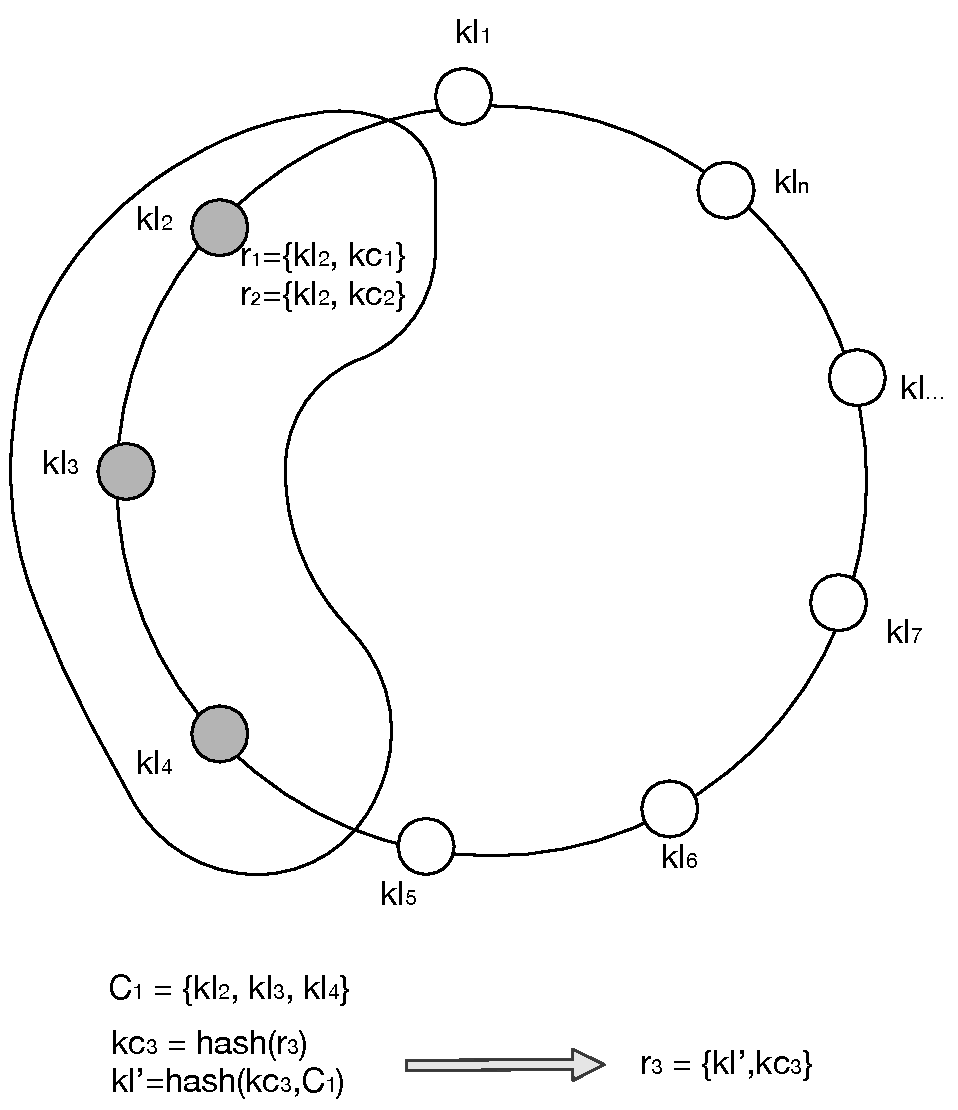
\includegraphics[width=0.5\linewidth]{img/hashing.pdf}
	%\vspace{-0.2cm}
	\caption{Cartographie des ressources renforçant la data-locality}
	\label{fig:hash}
	%\vspace{-0.2cm}
\end{figure}

Comme la clé de localisation se trouvera parmi les n{\oe}uds de la communauté, on augmente la probabilité de trouver la copie primaire dans les n{\}oe}uds concernés. De plus, cette stratégie n'empêche pas la réplication des données sur d'autres n{\oe}uds, garantissant la persistance des données en cas de défaillances. Cette approche est aussi tolérante aux variations du nombre de membres de la communauté : en cas de disparition d'un n{\oe}ud, c'est une réplique qui prend le relais ; en cas d'un nouveau membre, celui-ci sera intégré à la fonction de hachage normalement.   

\section{Exemples d'Utilisation de CloudFIT}

En tant que plate-forme expérimentale pour le calcul distribué et le \textit{fog computing}, CloudFIT est en constante évolution. Cela n'empêche pas son utilisation comme plate-forme de calcul dans certains de nos projets, notamment ceux dont l'objectif est d'utiliser des réseaux avec des éléments volatiles ou avec des ressources hétérogènes. Le premier exemple ci-dessous illustre une utilisation "recherche" pour le projet STIC-AmSud PER-MARE, dans le but d'évaluer le comportement de CloudFIT en tant que plate-forme \textit{MapReduce} pour les environnements pervasifs. Le deuxième exemple démontre une utilisation "production", où CloudFIT a été utilisé pour exécuter un workflow destiné aux sciences de l'atmosphère. Ce dernier travail a servi de base  pour la proposition du projet de collaboration CAPES-Cofecub MESO. 


\subsection{L'application WordCount}

Le projet STIC-AmSud PER-MARE (\textit{Adaptive Deployment of MapReduce-based Applications over Pervasive and Desktop Grid Infrastructures}) avait pour but le développement de stratégies pour le déploiement d'applications \textit{MapReduce} sur des environnements pervasifs. Si l'un des volets du projet a été celui d'adapter Apache Hadoop (voir la Section \ref{sec:Guilherme}), l'autre volet consistait à utiliser CloudFIT en tant que plate-forme de calcul distribuée. Si dans l'article présenté à CLIoT 2015 \cite{Steffenel15Taormina} nous nous sommes concentrés sur la performance de CloudFIT (voir aussi la Figure \ref{fig:Hadoop}), le travail présenté à CN4IoT \cite{Steffenel2015Roma} analysait l'exécution de CloudFIT par rapport à la volatilité et l'hétérogénéité des ressources.

\subsubsection{Impact de la volatilité}

Cette première expérience illustre le déploiement d'une application \textit{MapReduce} simple (\texttt{WordCount}) sur un corpus de textes faisant 1 GB de données et réparti en blocs uniformes de 64 MB. Cette répartition vise à reproduire le comportement de Hadoop, qui lui aussi traite les données par blocs de 64 MB.  Aussi afin de rendre la visualisation des expériences plus simple, les n{\oe}uds sont identiques et ont été explicitement limités à une seule exécution simultanée (un seul \texttt{Worker}). 

Dans un premier moment et afin d'avoir un barème de comparaison, la Figure \ref{fig:regular} présente le diagramme de Gantt pour une exécution sans incidents.
Nous pouvons avoir un aperçu du mécanisme d'ordonnancement distribué par défaut de CloudFIT, déjà discuté en Section \ref{subsec:commCloudFIT}. En effet, lorsque la liste de tâches est reçue par le TaskScheduler, celle-ci est réordonnée de manière aléatoire. L'ordonnanceur choisit ainsi la première tâche disponible (marquée "\textit{NEW}") et avertit les autres n{\oe}uds que cette tâche est en exécution. De manière similaire, à la fin de son exécution son statut est diffusé pour annoncer la fin de la tâche. Si toutes les tâches "\textit{NEW}" ont déjà été prises, un n{\oe}ud peut lancer des tâches spéculatives parmi celles marquées "\textit{STARTED\_DISTANT}". 

Plus spécifiquement, nous pouvons observer le déploiement des tâches \textit{map} (lesquelles ont des temps d'exécution variable selon le nombre de mots dans les documents), plus une tâche \textit{reduce} qui s'exécute à la fin. Bien que l'exemple \texttt{WordCount} ne contienne qu'une tâche Reduce, celle-ci se trouve exécutée par tous les n{\oe}uds car si le premier n{\oe}ud a marqué la tâche comme "\textit{STARTED}" et prévient les autres, ceux-ci n'ont rien de plus dans leur file d'exécution et lancent le Reduce en tant que tâche spéculative. Ceci n'a aucun impact sur le résultat final de l'application car les n{\oe}uds vérifient la présence d'un fichier de sortie avant de l'écrire sur la DHT, empêchant tout écrasement ou corruption. 

\begin{figure}
	\centering
		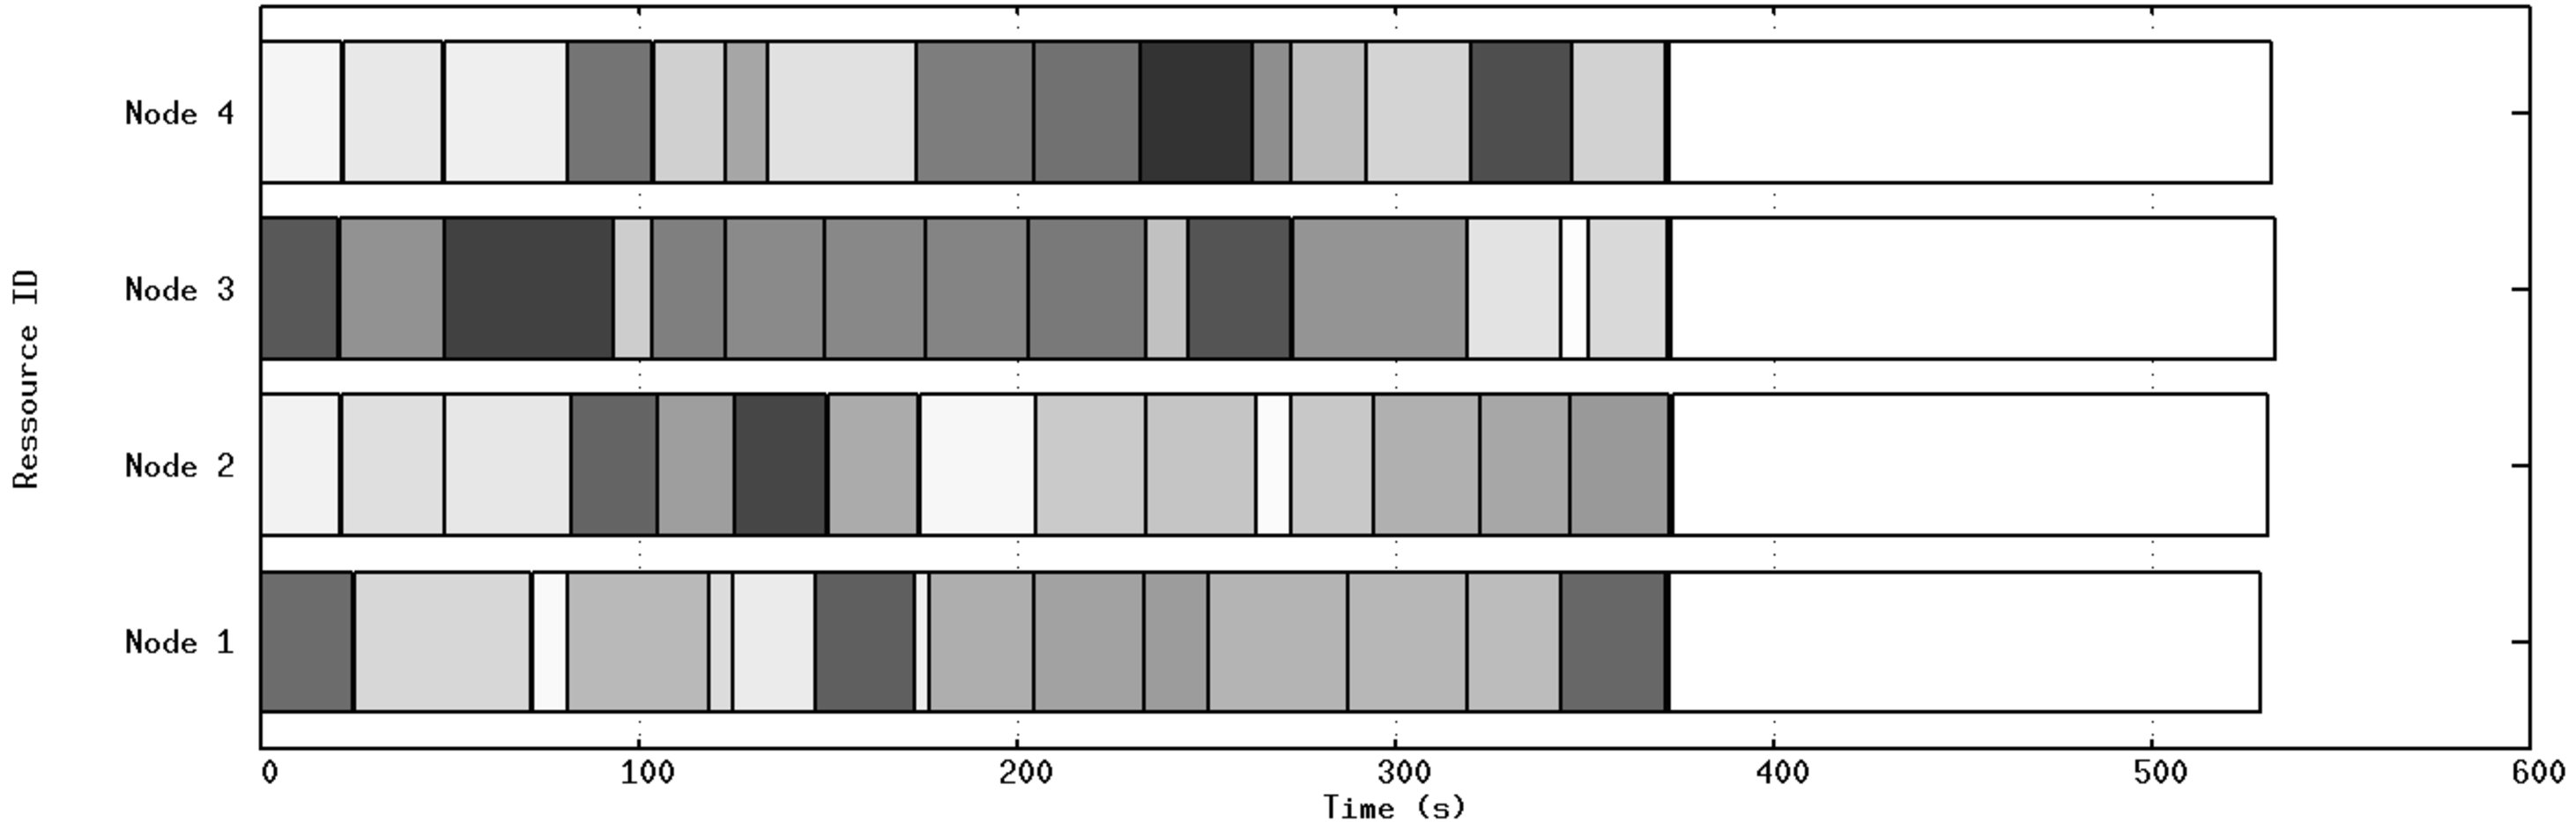
\includegraphics[width=1\linewidth]{img/regular2}
		\caption{Exécution de WordCount sur un cluster uniforme (1 GB de données en blocs de 64MB)}\label{fig:regular}
\end{figure}




Grâce à ces échanges, il est aussi possible de compléter les tâches initiées par les n{\oe}uds en défaillance ou mettre au courant un n{\oe}ud qui vient de rejoindre une communauté CloudFIT. La Figure \ref{fig:1out} représente ainsi une situation où un n{\oe}ud tombe en panne, avec la subséquente reprise des tâches par les autres n{\oe}uds. La Figure \ref{fig:reprise} va au-delà de cette situation en rajoutant un nouveau n{\oe}ud, qui récupère l'état actuel des tâches et peut ainsi contribuer avec l'effort de calcul.
\begin{figure}
	\centering
		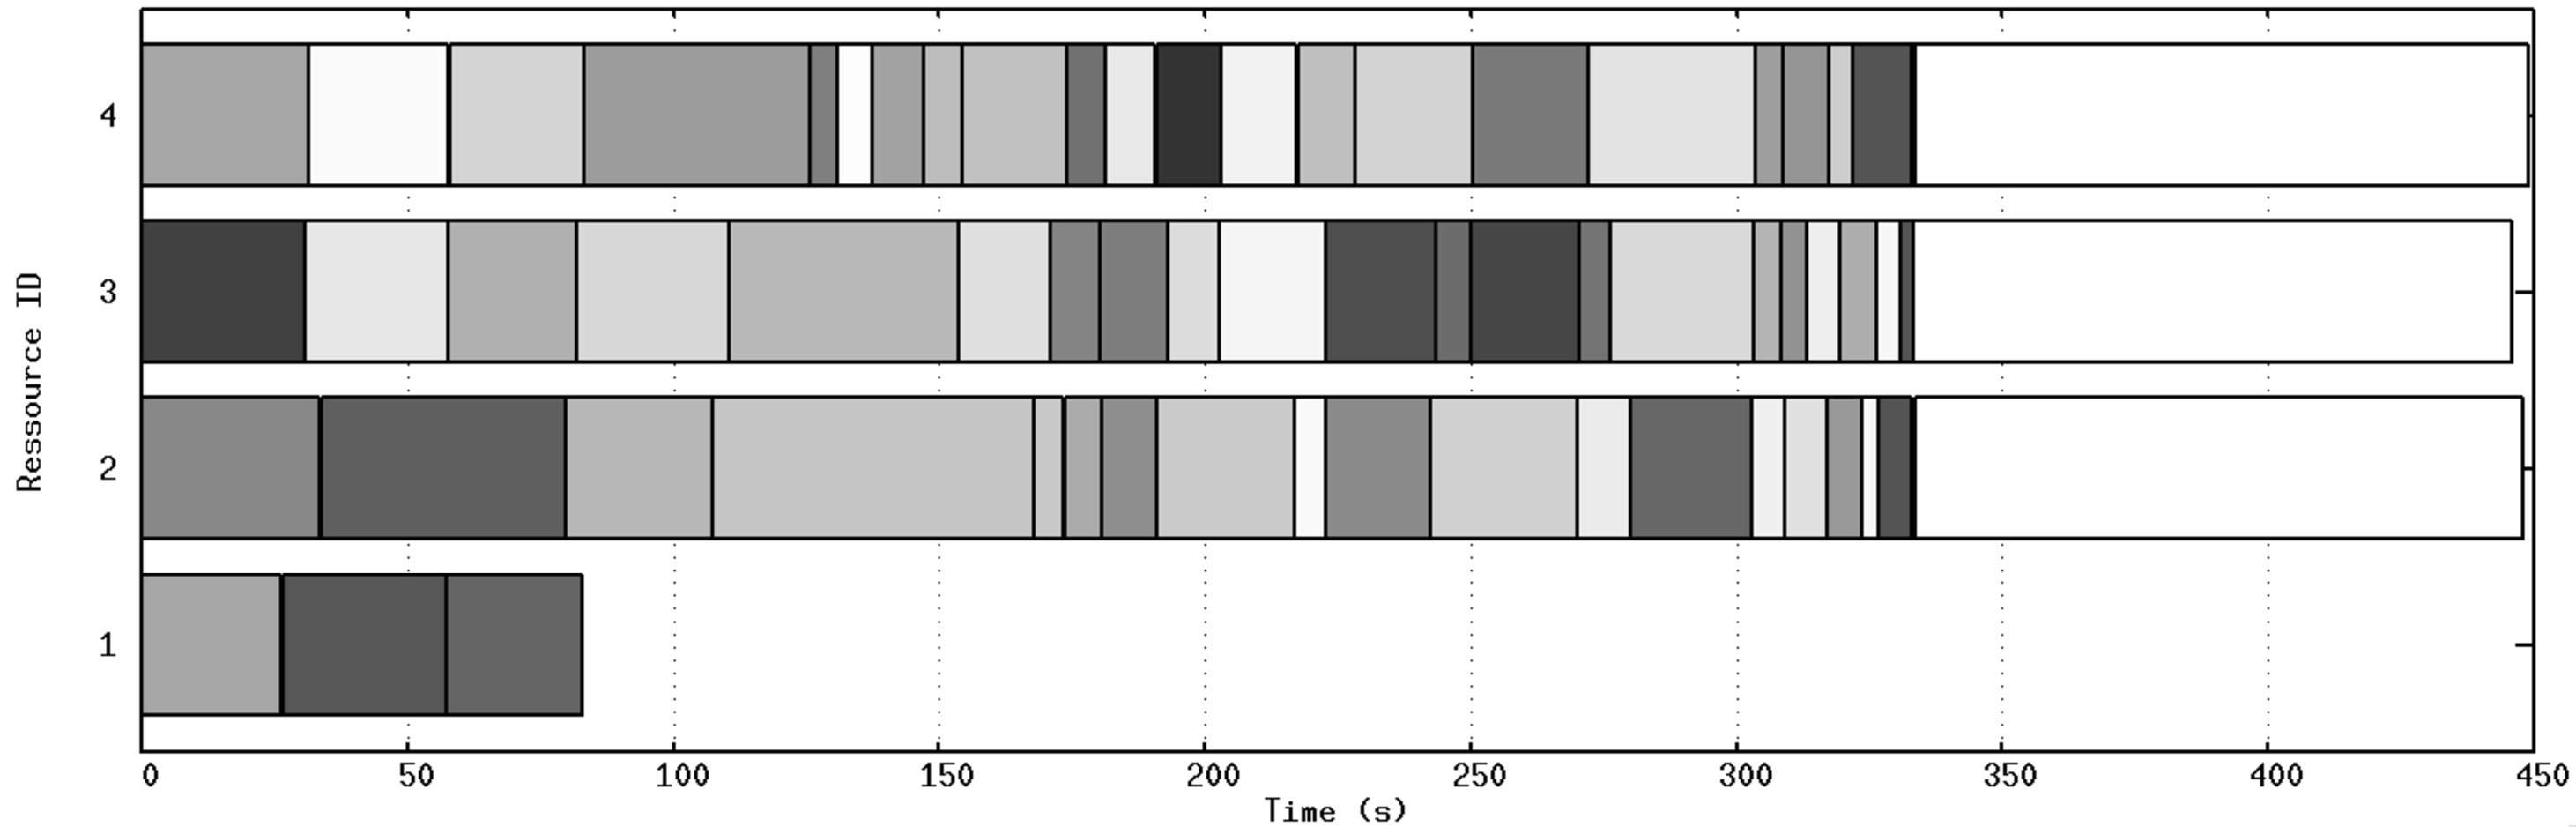
\includegraphics[width=1\linewidth]{img/1out2}
		\caption{Exécution de WordCount lorsqu'un n{\oe}ud disparaît (1 GB de données en blocs de 64MB)}\label{fig:1out}
\end{figure}

\begin{figure}
	\centering
		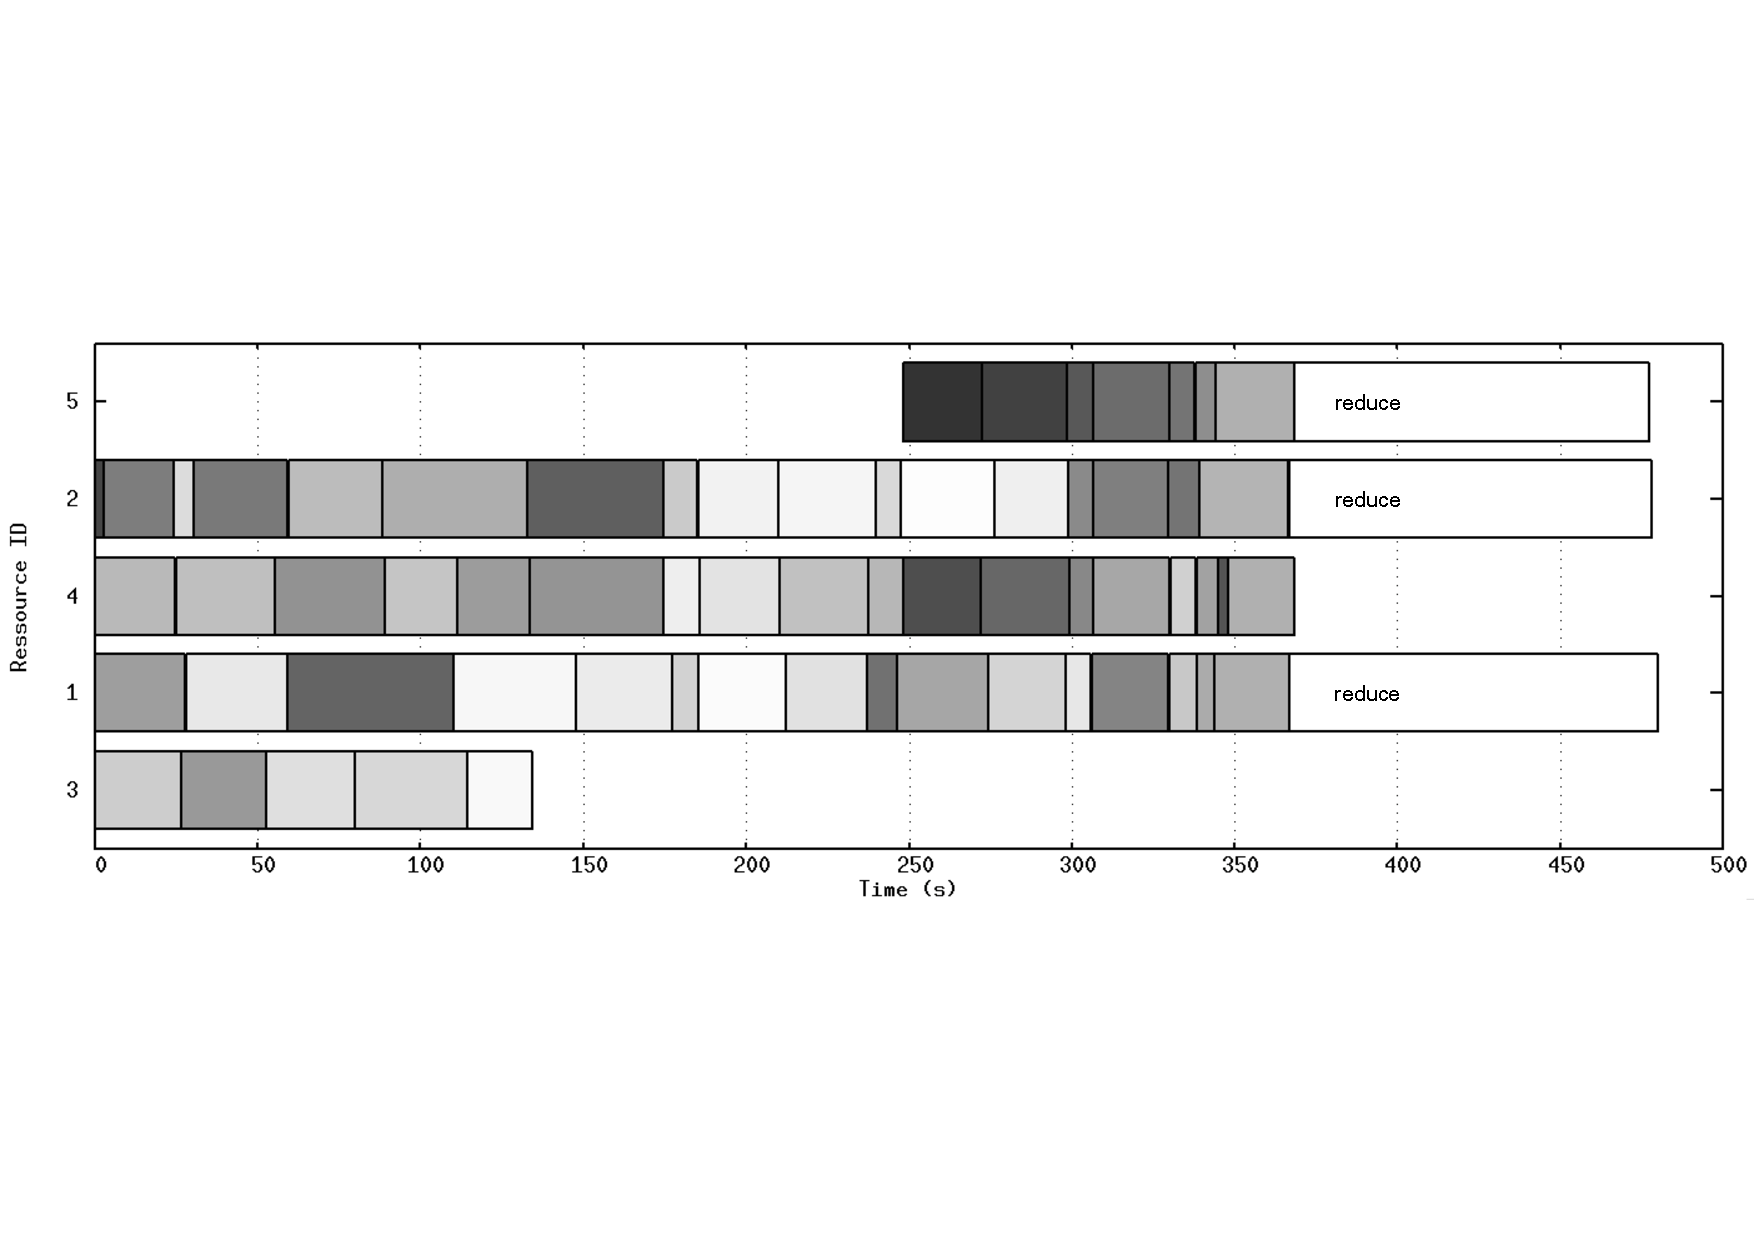
\includegraphics[width=1\linewidth]{img/reprise2}
		\caption{Exécution de Wordcount lorsqu'un n{\oe}ud rejoint la communauté après la défaillance d'un autre n{\oe}ud (1 GB de données en blocs de 64MB)}\label{fig:reprise}
\end{figure}


\subsubsection{Impact de l'hétérogénéité}

Cette deuxième expérience vise l'observation de CloudFIT dans un environnement hétérogène. Pour cela, nous avons interconnecté quatre n{\oe}uds avec des spécifications assez différentes (cf. le Tableau \ref{Table:laptops}). Comme dans l'expérience précédente, nous limitons le nombre de c{\oe}urs (\texttt{Workers}) sur les machines pour rendre la visualisation plus simple.

\begin{table}
	\begin{center}
		\begin{tabular}{|c|c|c|c|c|c|c|}
			\hline
			Type de N{\oe}ud & Processeur & GHz &  Mémoire & OS\\
			\hline
			\hline
			MacBook Air & Intel Core i7-4650U & 1.7   & 8 GB & MacOS 10.10.5 \\
			Lenovo U110 & Intel Core2 Duo L7500 & 1.6   & 4 GB & Ubuntu Linux 15.4 \\
			Raspberry Pi 2 & ARM Cortex-A7 & 0.9  & 1 GB & Raspbian Linux Wheezy\\
			VM Virtualbox & Intel Core i7* & 2.2*  &  1 GB & Debian Linux 8.2 \\
			\hline
			\multicolumn{5}{l}{* ces valeurs sont celles vues par la machine virtuelle}
		\end{tabular}
	\end{center}
	\caption{\label{Table:laptops}Spécification des n{\oe}uds du cluster pervasif}
\end{table} 

Nous avons aussi modifié les paramètres de l'expérience afin d'exécuter le WordCount sur 512MB de données divisées en petits blocs de 2MB seulement ; nous pensons que cette configuration est plus proche de celle rencontrée lors de la transmission de données par les dispositifs IoT. La multiplication de tâches avec un coût individuel plus réduit rend aussi possible la participation des n{\oe}uds avec moins de puissance de calcul.  La Figure \ref{fig:hetero} affiche le diagramme de Gantt pour une exécution de ce scénario. 

\begin{figure}
	\centering
		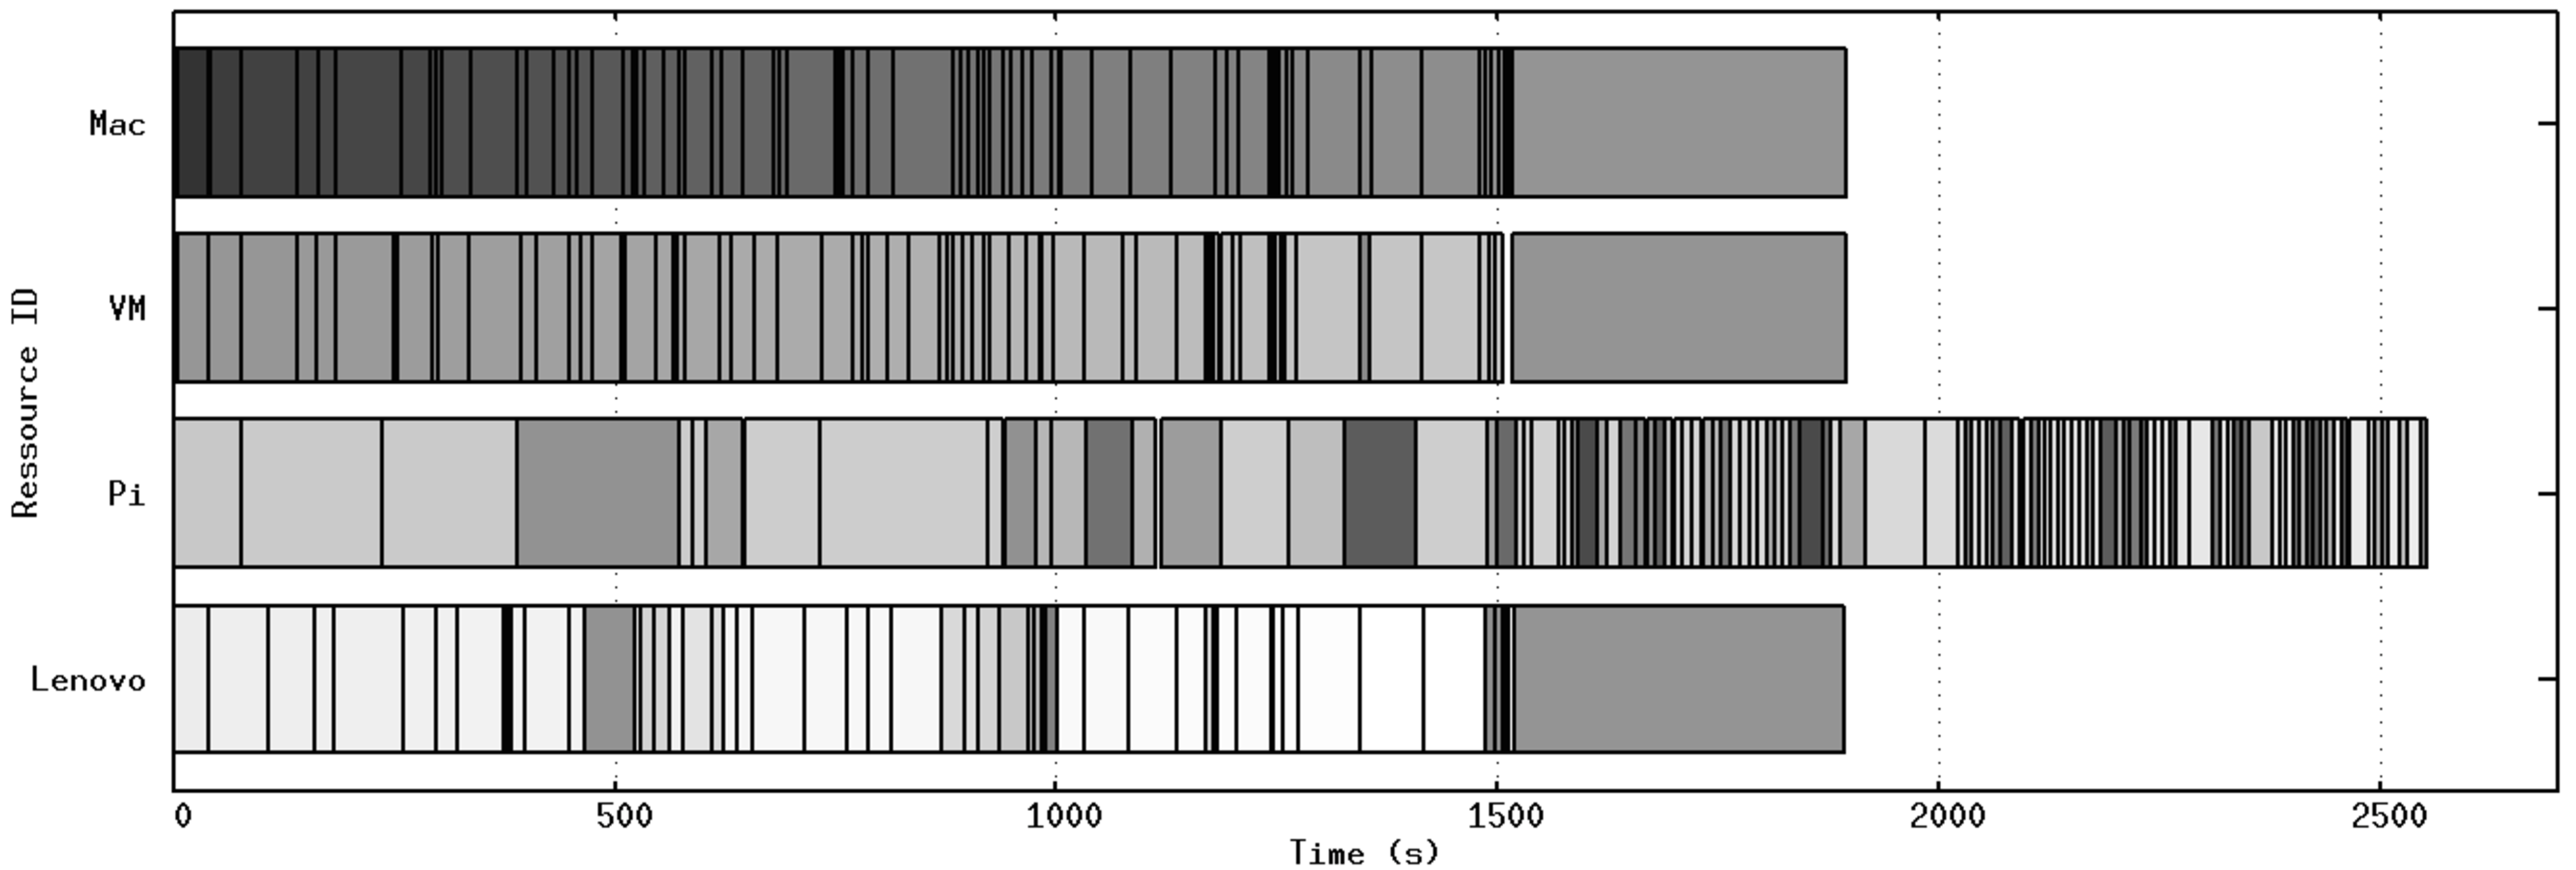
\includegraphics[width=1\linewidth]{img/hetero2}
		\caption{Exécution de Wordcount dans un cluster hétérogène (512MB en blocs de 2MB)}\label{fig:hetero}
\end{figure}

Alors que la répartition des tâches entre les notebooks et la machine virtuelle ne présentent pas une différence significative, le Raspberry Pi, sans surprise, n'arrive pas à exécuter les tâches aussi vite que les autres n{\oe}uds (voir la longueur des tâches dans la première partie de l'exécution). De plus, ce n{\oe}ud est tellement surchargé qu'il perd plusieurs messages de mise à jour et ne détecte pas la fin de la phase \textit{map}. Comme résultat, il essaye vainement d'exécuter toutes les tâches juste pour se rendre compte que leur résultat est déjà dans la DHT, la raison pour la petite durée des tâches vers la fin (cette vérification préalable était prévue pour éviter le travail en doublon et les risques de corruption des données). 

Au lieu de freiner notre intérêt par les dispositifs de faible puissance, ces résultats nous incitent à vouloir comprendre les raisons de ces problèmes. En effet, les dispositifs de faible puissance tels que les Raspberry Pi n'ont pas seulement des processeurs moins rapides mais aussi des limitations sur la taille et la vitesse d'accès à la mémoire et au stockage (quelques centaines de MB de RAM, des mémoires SD à la place des disques durs, etc.). Dans ces dispositifs, les tâches de gestion de l'overlay P2P et de la DHT (par exemple, la réplication des données) peuvent occuper une partie importante de leurs ressources et finir par interférer avec le traitement des messages échangé via l'overlay.  Ces résultats ont motivé la mise en place des stratégies de collecte de contexte pour un meilleur ordonnancement et aussi les méthodes d'optimisation du stockage que nous avons détaillé dans la section précédente. 

\subsection{Détection d'Événements Secondaires de la Couche d'Ozone}

La découverte du trou d'Ozone de l'Antarctique \cite{Farman1985} a galvanisé l'intérêt de la communauté scientifique et depuis ce moment plusieurs études ont été menées dans le but de surveiller la variation de la densité de la couche d'Ozone sur les régions polaires \cite{Solomon1999}\cite{Salby2012}. La réduction de la couche d'Ozone peut aussi déclencher plusieurs événements sur des zones situées à des latitudes moyennes, soit à cause du mouvement de la bordure du vortex polaire sur ces régions  \cite{Kirchhoff1997}\cite{Marchand2005} ou bien à cause du transit de masses d'air pauvres en Ozone détachées du vortex polaire. Ce dernier cas est appelé "événements dus à l'influence du trou d'ozone Antarctique", ou plus simplement des Événements Secondaires de l'Ozone" (\textit{Ozone Secondary Events}  - OSE). 

Causés par la circulation de l'atmosphère, ces masses d'air continuent à se déplacer pendant 7 à 20 jours après leur séparation du vortex polaire et peuvent atteindre des latitudes plus élevées, occasionnant une réduction temporaire de la colonne totale d'Ozone (\textit{Total Column Ozone} - TCO) sur des zones qui sont souvent habitées \cite{Prather1990}\cite{Waugh1994}\cite{Manney1994}. Comme résultat, des niveaux élevés de radiation ultraviolet nocive (UVB et UVC) atteigne la surface \cite{Casiccia2008}, à un tel point qu'une réduction de 1\% de la colonne totale d'Ozone peut occasionner une augmentation de 1.2\% de la radiation UV mesurée sur le sud du Brésil \cite{Guarnieri2004}. Ces événements secondaires de l'Ozone sont régulièrement observés sur des zones peuplés en moyenne latitude, comme par exemple en Amérique du Sud \cite{Kirschhoff1996}\cite{Pinheiro2011}, en Afrique du Sud \cite{Semane2006}\cite{Sivakumar2007}, à la Nouvelle Zélande \cite{Brinksma1998} et aussi sur l'Île de la Réunion \cite{toihir2015}. 

%\begin{figure}
%	\centering
%	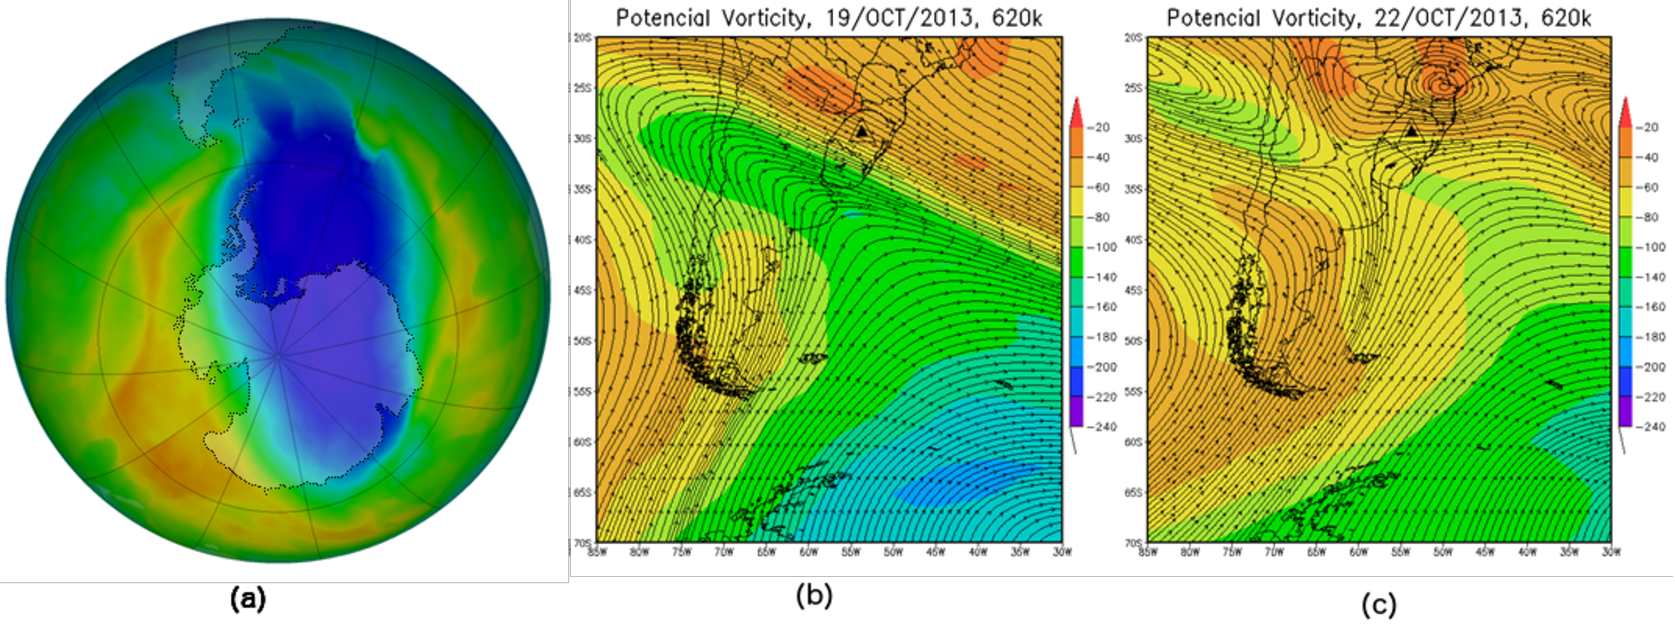
\includegraphics[width=0.75\linewidth]{img/22_10_13-c}
%	\vspace{-0.2cm}
%	\caption{OMI satellite image for 18 October 2013 (a) and the associated wind currents for (b) 19 and (c) 22 October 2013 at 620K}
%	\label{fig:event2013}
%	\vspace{-0.3cm}
%\end{figure}

Malgré une forte liaison avec la dynamique de la stratosphère, le nombre d'études visant la modélisation de la circulation dynamique de la couche d'Ozone sont encore très rares \cite{Marchand2005}. En effet, la plupart des modèles climatiques se limitent aux couches inférieures de l'atmosphère, notamment celles liées à aux prévisions météorologiques, et n'explorent pas les interactions avec les couches supérieures comme celle où se trouve la couche d'Ozone. Plus récemment, un modèle obtenu par Vaz Peres \cite{Peres2013} a permis une certaine compréhension de ces phénomènes. En se concentrant sur les données d'épisodes OSE déjà identifiés dans le passé, le modèle de Vaz Peres a permis la reproduction des événements observés. En partant de cette étude, notre but était d'utiliser des techniques du \textit{big data} et du \textit{data mining} afin de ramasser plus de données et extraire des modèles plus précis, permettant la prévision des occurrences de ces événements.

L'utilisation de techniques du \textit{big data} est essentiel car les données concernant la couche d'Ozone s'accumulent d'année en année. Par exemple, l'équipement TOMS/OMI placé dans les satellites de la NASA satellite produit plus d'1GB de données brutes par an. Juste les observations des satellites TOMS/OMI remontent à 1978 (ce qui fait presque 40 GB en ce moment), et à cela on peut rajouter d'autres sources de données satellites telles que les satellites de l'ESA mais aussi des observations effectuées au sol. 

\subsubsection{Identification des événements secondaires de l'Ozone avec CloudFIT\label{sec:development}}

Si dans un premier temps l'usage d'une plate-forme type cluster ou cloud pourrait être envisagée, notre attention s'est portée sur CloudFIT car celui-ci a l'avantage d'exploiter les ressources de calcul disponibles, sans obliger l'installation ou la maintenance d'un parc informatique dédié. En autre, le traitement des données et la détection des OSE varie selon la zone géographique couverte et selon le type d'analyse effectuée : la détection d'événements passés utilisée pour améliorer les modèles est assez simple, alors qu'une analyse plus poussée visant l'étude des corrélations entre les événements et les courants atmosphériques peut s'avérer bien plus demandeuse de ressources. L'utilisation de CloudFIT permet la création d'une plate-forme de calcul élastique.

Dans le cas précis de la détection des OSE, nous avons identifié quatre activités principales qui peuvent être transposées sur CloudFIT. Ces activités sont les suivantes : 
\begin{enumerate}
	\item \textbf{Pré-traitement des données} - transformation des données brutes OMI ;
	\item \textbf{Filtrage et agrégation} - sélection des données concernant une zone géographique et une période donnée, puis des opérations d'agrégation si nécessaire ;
	\item \textbf{Extraction des paramètres} - extraction des moyennes et écarts types pour une région et une période donnée ;
	\item \textbf{Détection des événements} - identification des valeurs anormales d'Ozone, génération d'alertes.
\end{enumerate}

Le pré-traitement des données est nécessaire car les données brutes fournis par l'équipement TOMS/OMI sont dans un format difficile à utiliser. Le filtrage permet de limiter la recherche sur une zone géographique et/ou sur une période d'étude, alors que l'agrégation permet l'obtention de données à une granularité différente de celle d'origine (utile notamment pour la corrélation avec d'autres types de données). En effet, la plupart des données TOMS/OMI ont une résolution d'1 dégrée, alors que d'autres sources de données ont parfois des cartographies plus détaillées (par exemple, avec 0.25 dégrée d'arc entre chaque mesure). Cette procédure sera détaillée dans la section suivante.

L'extraction des paramètres est la prochaine étape car la détection d'un OSE est liée à l'observation d'une chute anormale de la concentration de l'Ozone. Pour cela, il faut extraire des paramètres historiques tels que la moyenne et la variation (écart-type), et cela pour chaque coordonnée analysée. Cette procédure est aussi détaillée dans les sections suivantes. Finalement, la détection se fait en comparant la mesure d'un instant précis avec la série temporelle des journées précédentes. Si les valeurs sont inférieures à la variation normale de la période, alors on peut déclencher une procédure d'alerte, signalant aux autorités sanitaires un risque lié à la radiation UV qui menace la population.

Les trois premières activités sont des exemples d'opérations ETL (\textit{Extract, Transform, Load}) typiques du \textit{big data}. La dernière activité peut être considérée comme un algorithme de prise de décisions. Nous avons donc établi un workflow qui peut être transcrit comme un enchaînement de jobs CloudFIT, comme illustré en Figure \ref{fig:blocs}. Par conséquent, les quatre premiers jobs (Preprocess, Filtering, Time-series et Detection) peuvent même être exécutés sur des communautés CloudFIT différentes : des équipements entrée de gamme regroupés en Community C1 peuvent être utilisés pour pré-traiter et stocker les données des satellites et des spectre-photomètres Brewer ou Dobson installés au sol. 

Par la suite, les données peuvent donc être traitées pour la détection ou bien être utilisées pour des analyses plus poussées telles que la recherche de motifs récurrents ou la prévision d'événements futurs. Les activités telles que le filtrage et l'analyse des séries temporelles demandent des ressources de calcul plus importants, fournis par la communauté C2.
La Figure \ref{fig:blocs} inclut aussi d'autres communautés (C3 et C4) qui pourraient être déployées séparément afin d'effectuer les autres activités liées à la détection et à la prévision des OSE (ces étapes n'ont pas été implémentées). Il faut noter que cette organisation répond aussi aux principes du calcul multi-échelle et du \textit{fog computing}, l'un des objectifs de CloudFIT.

\begin{figure}
	\centering
	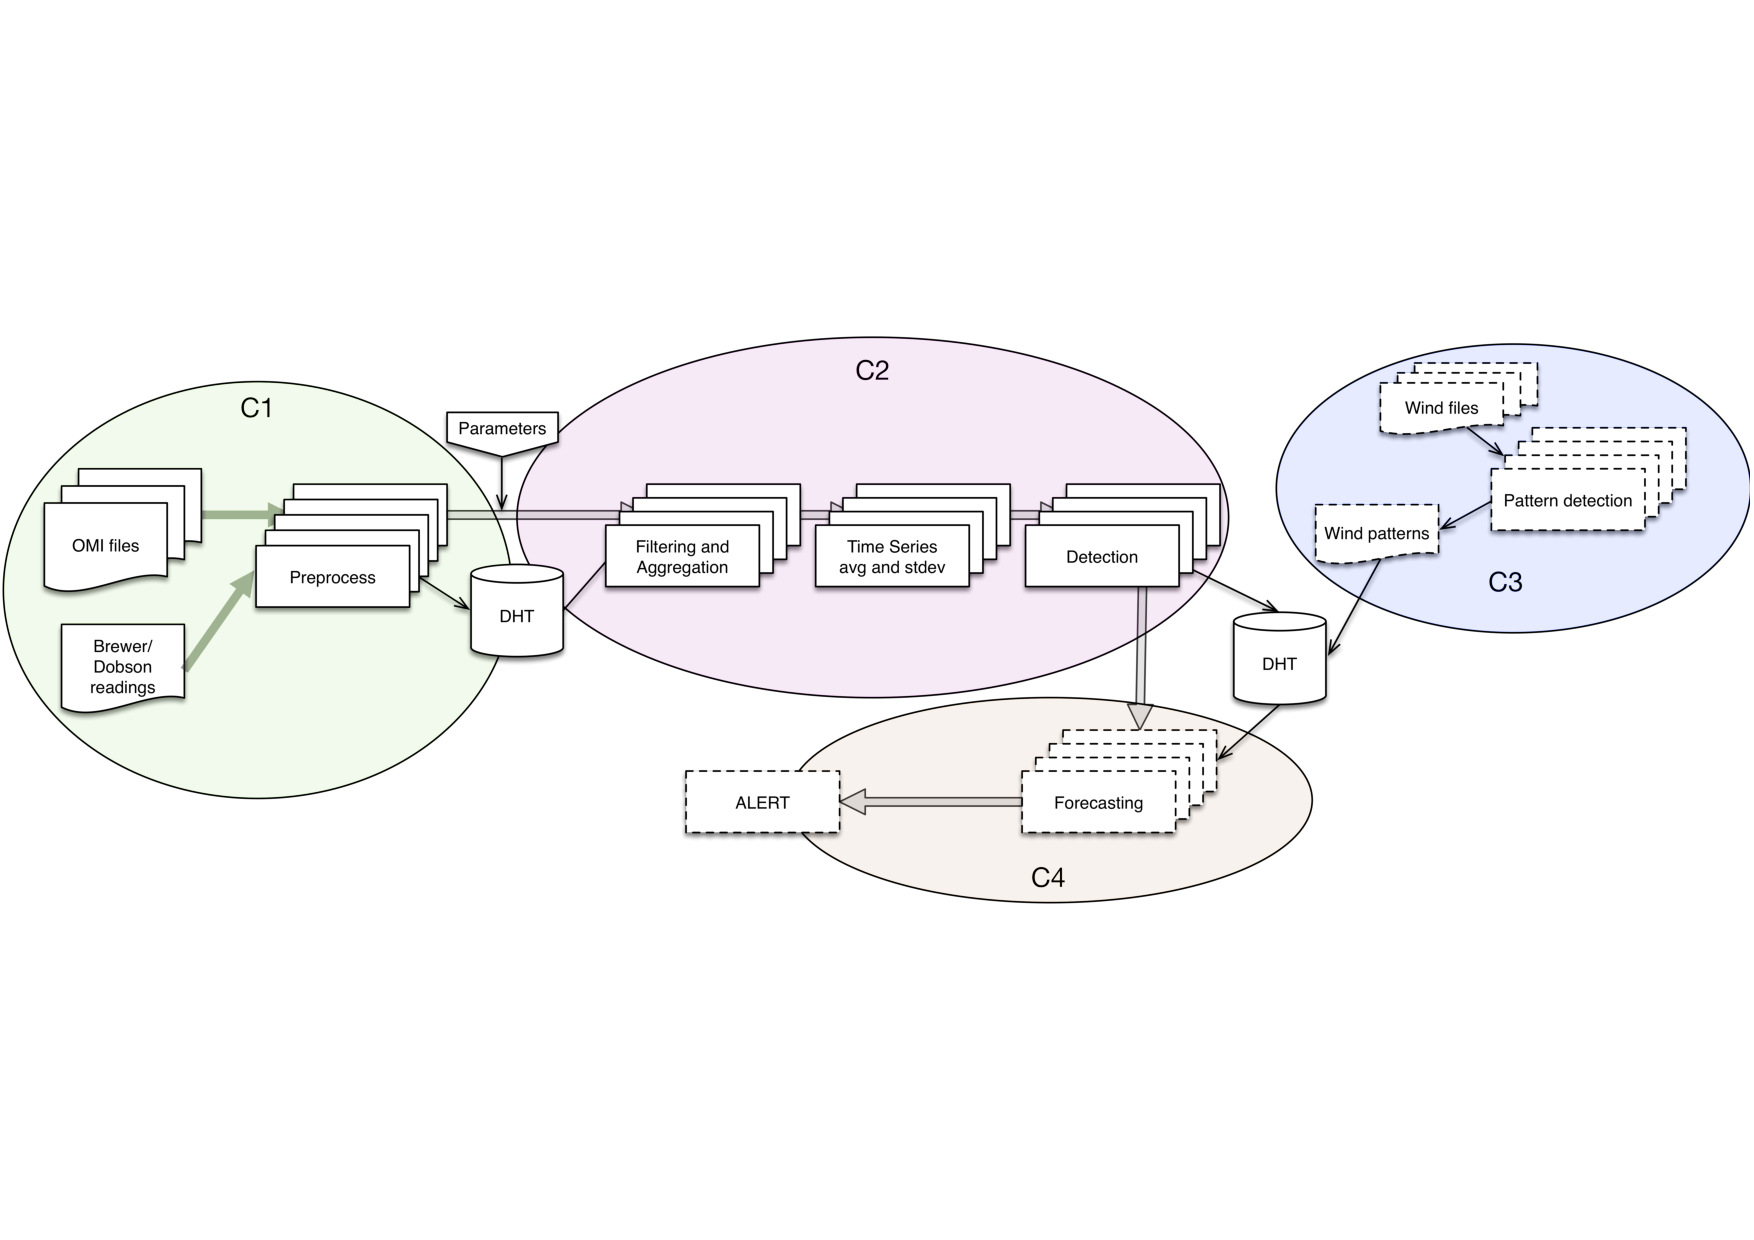
\includegraphics[width=1\linewidth]{img/4-process}
	\caption{Organisation des activités dans un réseau CloudFIT}\label{fig:blocs}
\end{figure}

\subsubsection{Pré-traitement des données}

Les mesures de la colonne totale d'ozone peuvent être obtenues par des équipements au sol mais aussi par le biais des satellites, qui ont l'avantage d'offrir une couverture globale. L'un de ces équipements, l'instrument TOMS/OMI, rend publique les données consolidées de la couverture du globe, une fois par jour. Dans le cas de la détection des événements secondaires de l'Ozone, nous avons besoin des données brutes obtenus par les satellites. Ces données sont présentées selon le format illustré en Figure \ref{fig:toms}(a), ce qui n'est pas vraiment adapté à l'utilisation direct pour nos calculs. Chaque fichier contient un entête avec des informations sur le fichier (date, les coordonnées du grillage, le pas), suivi des mesures pour chaque latitude (indiquée à la fin de la ligne), et cela pour toutes les longitudes couvertes. Chaque mesure est exprimée en unités Dobson (UD), représentées par un entier à 3 chiffres qui doit être séparé des mesures des autres longitudes. Par exemple, les coordonnées (-89.5,-179.5) de la Figure \ref{fig:toms}(a) ont la valeur 280, les coordonnées (-89.5,-178.5) ont aussi la valeur 280, et ainsi de suite.   

\begin{myverbbox}[\tiny]{\TOMS}
	Day:   1 Jan  1, 2013    OMI TO3    STD OZONE    GEN:13:003 Asc LECT: 01:44 pm 
	Longitudes:  360 bins centered on 179.5  W  to 179.5  E   (1.00 degree steps)
	Latitudes :  180 bins centered on  89.5  S  to  89.5  N   (1.00 degree steps)
	280280280280280280280280280280280280280280280280280280280279279279279279279
	279279279279279279279279279279279279279279279279279279279279279279279279279
	279279279279279279279279279279279279279279279279279279279279279279279279279
	279279279279279279279279279279279279279279279279279279280279280280280280280
	280280280280280280280280280280280280280280280280280280280280280280280280280
	280280280280280280280280280280280280280281281281281281281281281281281281281
	(...)
	282282282282282282282282282282   lat =  -89.5
	(...)   lat =  -88.5
	(...)   lat =  -87.5
	(...)
\end{myverbbox}

\begin{myverbbox}[\tiny]{\JSON}
	{
		"date":"20130101",
		"step":"1.0",
		"latitudes":{
			"-89.5":["-179.5":"280","-178.5":"280",(...)],
			"-88.5":["-179.5":"272","-178.5":"272",(...)],
			(...)
		}
	}
\end{myverbbox}

\begin{figure}
	\centering
	\begin{tabular}{cc}
		\imagetop{\TOMS}&\imagetop{\JSON}\\
		{\small (a)}&{\small (b)}
	\end{tabular}
	%\vspace{-0.2cm}
	\caption{Fichier brute OMI Ozone (a) et sa représentation JSON (b)}\label{fig:toms}
	%\vspace{-0.3cm}
	
\end{figure}

Comme ce format est difficile à comprendre et à traiter (il faut parcourir l'ensemble des entrées d'une latitude pour obtenir une mesure à une longitude donnée), nous avons décidé de pré-traiter ces fichiers et les stocker sur la DHT en tant que objets JSON, selon le \textit{template} présenté en Figure \ref{fig:toms}(b). JSON est un format structuré de données bien connu, qui peut être facilement requêté, importé sur des bases de données ou bien stocké directement dans des bases NoSQL orientées  documents. Le pré-traitement est facilement parallélisable car chaque journée peut être traitée indépendamment des autres. De plus, le stockage sur une DHT permet la réutilisation de données déjà traitées et l'ajout de nouvelles entrées à chaque jour. 

\subsubsection{Analyse des séries temporelles et la détection des OSE\label{sec:timeseries}}

Comme indiqué précédemment, les OSE peuvent être détectés par des réductions anormales de la colonne totale d'Ozone alors que cela n'est pas directement lié à l'expansion du trou de la couche d'Ozone Antarctique. Cette détection est faite par la comparaison entre la mesure d'une journée et les moyennes historiques pour cette région. Cependant, le choix de ce qu'on considère la "période historique" a un impact important sur la perception des événements. Pour commencer, on ne peut pas utiliser la moyenne annuelle car la concentration d'Ozone varie saisonnièrement (dans l'hémisphère sud elle est plus basse à l'Automne et plus haute au Printemps). 

L'approche utilisé par Perez \textit{et al. }\cite{Peres2013} considérait la moyenne historique mensuelle, i.e., la moyenne historique de chaque mois des années enregistrées. De cette forme, une mesure effectuée le 2 Octobre et l'autre le 30 Octobre seraient comparées à la moyenne historique du mois d'Octobre. Si cela permet déjà la détection de certains OSE, cette méthode n'est pas suffisamment précise car la concentration naturelle varie d'année en année et aussi parce que la variation entre le début et la fin d'un mois est très importante dans les mois de transition comme Juillet ou Novembre. L'utilisation d'une moyenne standardisée aurait comme conséquence un nombre important de faux-positifs et faux-négatifs. Vu que nous disposons de ressources de calcul, nous avons décidé d'utiliser une approche par fenêtres glissantes, où par exemple chaque mesure est comparée à la moyenne des 15 jours précédents. Cette solution (l'utilisation de \textit{time series}) est plus proche de la réalité et prend en compte la variation naturelle pour la période étudiée.

Comme pour le pré-traitement des fichiers d'entrée, cette activité peut être exécuté en parallèle car chaque coordonnée (X, Y) a son propre ensemble de données. De même, le calcul de la moyenne et de l'écart type est indépendant pour chaque jour choisi, vu que la fenêtre glissante couvre des dates différentes. Ainsi, dans l'implémentation CloudFIT, les tâches de calcul sont définies en fonction du nombre de coordonnées. Chaque tâche lit les valeurs pour les 15 jours précédents et calcule la moyenne et l'écart type. Par exemple, si nous considérons la zone couverte par les coordonnées \{(-70.5, -84.5), (-20.5, -29.5)\} (les mêmes utilisées en Figure \ref{fig:progression}) avec un pas d'1 dégrée pour le grillage, nous avons 50x55 points à analyser (2750 tâches). 

Une fois obtenus la moyenne et l'écart type pour chaque coordonnée et pour chaque jour cible, la détection des OSE peut être effectuée.  Pour cela, nous utilisons la formule simple présentée en Équation \ref{eq:equation}. Cette formule considère qu'un OSE existe si la valeur mesurée est inférieure à un seuil déterminé en fonction de la moyenne des 15 derniers jours et de la latitude (dans le cas du sud du Brésil on considère ce seuil à $1.5 \times$ l'écart type). Des paramètres additionnels tels que la vorticité potentielle pourraient être rajoutés afin d'augmenter la précision des détections.

\begin{equation}
Detection(v)=\left\{ \begin{array}{c}
\begin{array}{lll}
\textbf{True} & &if \:\: v \:< (average - 1.5\times stdev)\\
\textbf{False} & &otherwise\end{array}\end{array}\right.
\label{eq:equation}
\end{equation}



\subsubsection{Résultats préliminaires}

Afin de valider l'implémentation, nous avons comparé les données de Peres \textit{et al.} \cite{Peres2013} avec les résultats obtenus à partir du workflow CloudFIT. Comme attendu, notre implémentation permet d'observer la progression du front OSE entre le 18 et le 22 Octobre 2013 (Figure \ref{fig:progression}). On observe que le mécanisme de détection mis en place permet de se concentrer uniquement sur les zones ayant subi une variation importante de la colonne d'Ozone et pas sur celles qui habituellement ont une concentration réduite (comme par exemple le pôle ou les régions australes de l'Argentine et du Chili). 

\begin{figure}
	\centering
	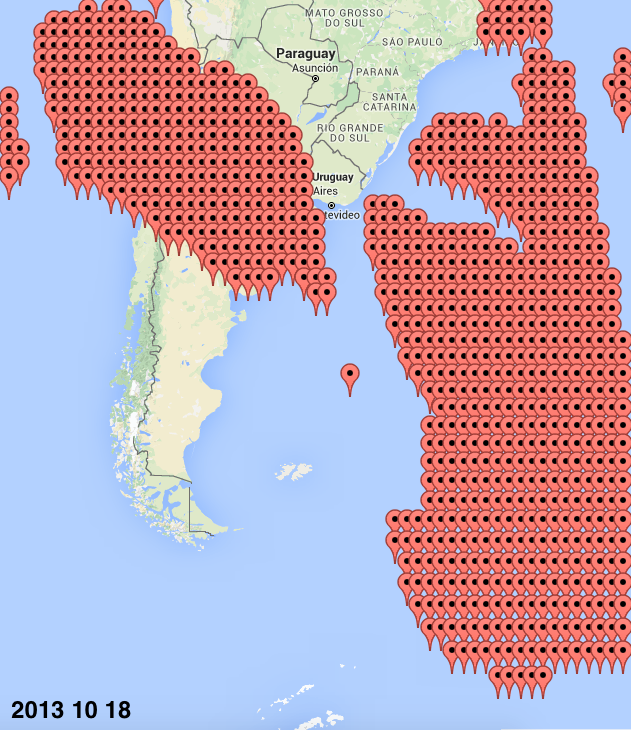
\includegraphics[width=0.19\linewidth]{img/20131018-b}~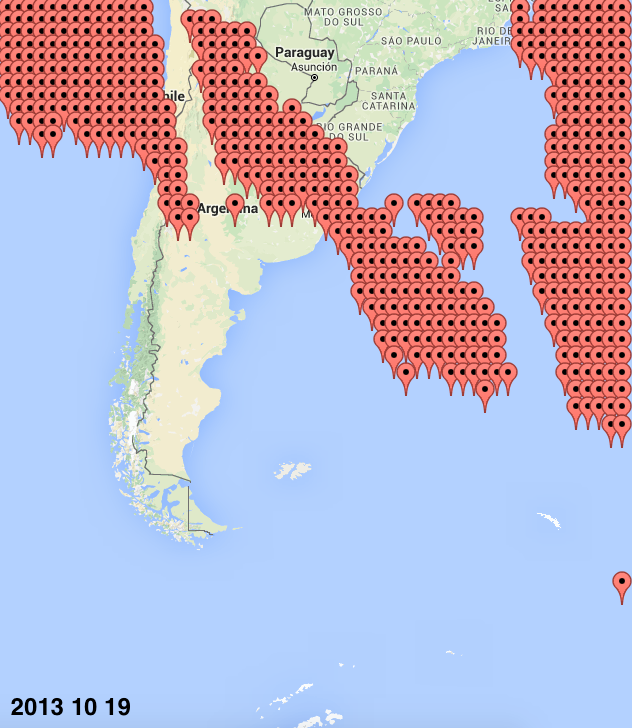
\includegraphics[width=0.19\linewidth]{img/20131019-b}~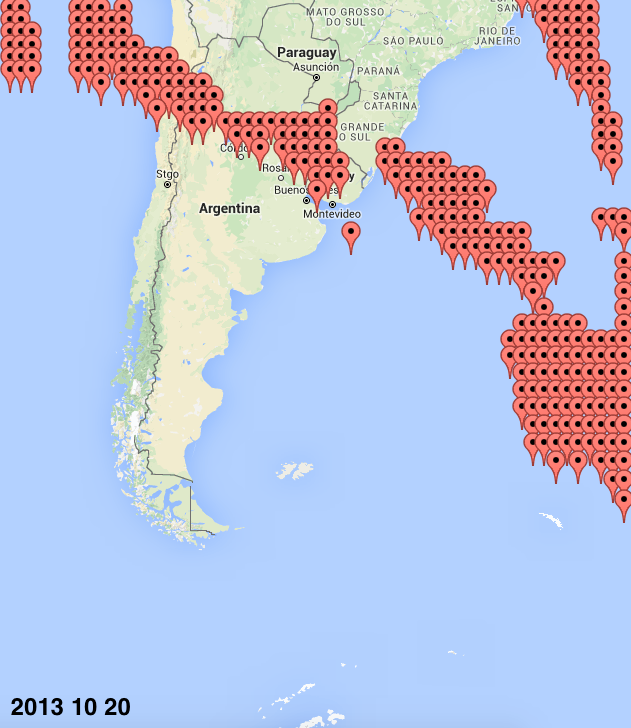
\includegraphics[width=0.19\linewidth]{img/20131020-b}~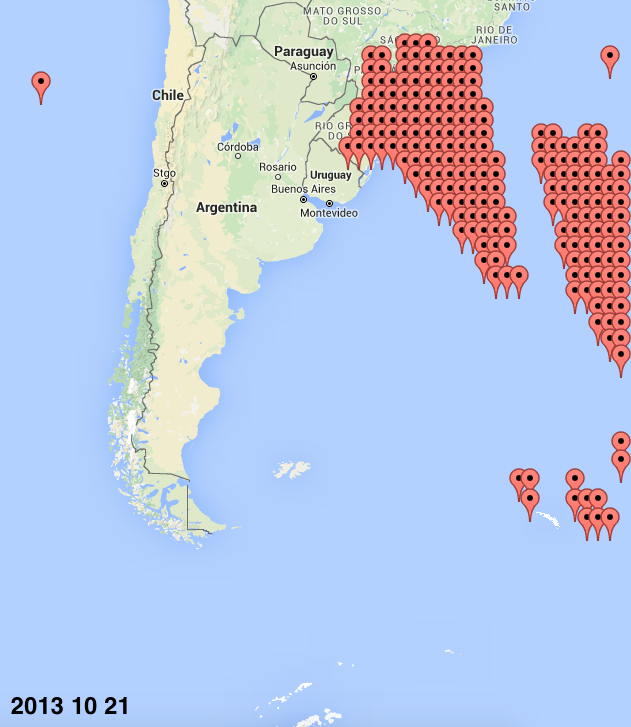
\includegraphics[width=0.19\linewidth]{img/20131021-b}~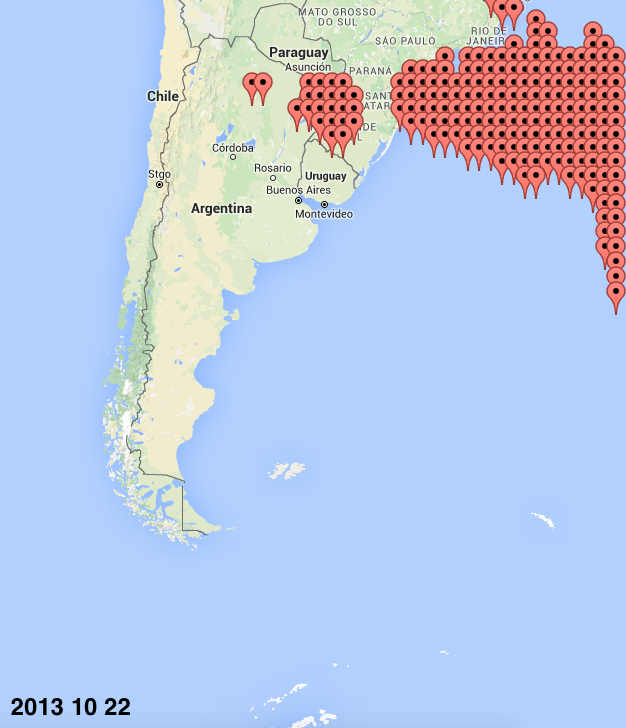
\includegraphics[width=0.19\linewidth]{img/20131022-b}
	%\vspace{-0.2cm}
	\caption{Progression de l'OSE observé entre le 18 et le 22 Octobre 2013}\label{fig:progression}
\end{figure}

Nous avons aussi comparé les coordonnées des OSE par rapport aux données de vorticité potentielle, l'un des facteurs étudiés par Peres. Afin de ne pas surcharger l'image, nous avons tracé seulement les points situés à proximité de l'observatoire de Santa Maria (Brésil). Comme montrent les cartes dans la Figure \ref{fig:comparison}, on observe une forte corrélation entre la vorticité potentielle et l'approximation des masses d'air pauvres en Ozone, spécialement sur la carte du 20 Octobre.  On peut aussi observer que ces OSE prennent du temps à se dissiper : même si la vorticité potentielle s'est déplacée, une poche pauvre en Ozone persiste sur une zone habitée deux jours plus tard. Ces résultats encouragent la poursuite de l'étude de la corrélation entre les OSE et la vorticité potentielle.


\begin{figure}
	\centering
	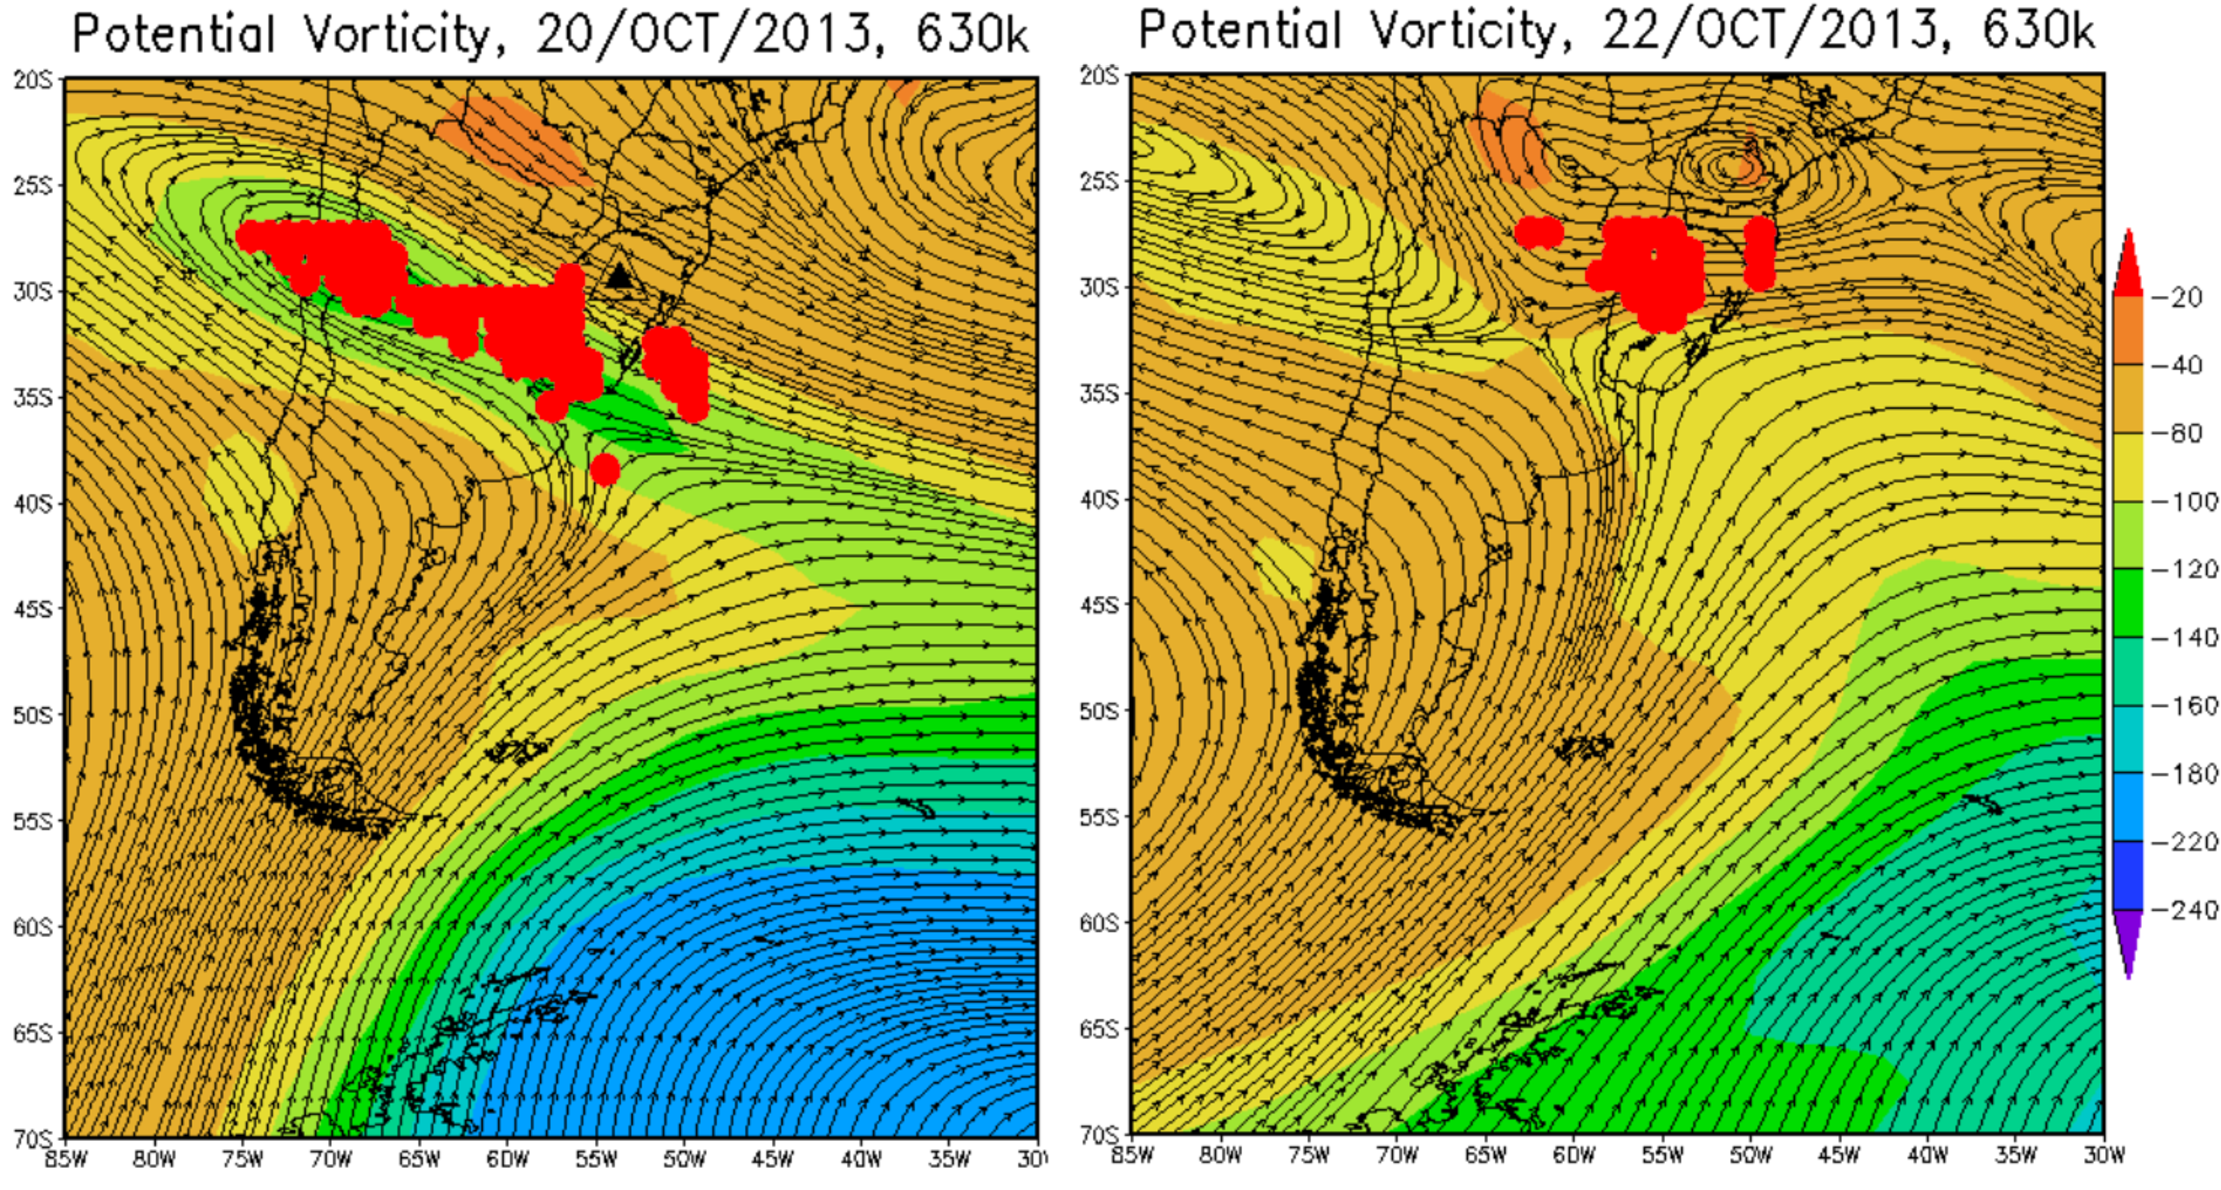
\includegraphics[width=0.55\linewidth]{img/comparison2}
	%\vspace{-0.2cm}
	\caption{Superposition des OSE identifiés sur Santa Maria, Brésil (29.68 S, 53.81 W)  et les cartes de la vorticité potentielle}\label{fig:comparison}
\end{figure}

La scalabilité de l'application a aussi été étudiée car cet algorithme peut être utilisé autant pour des détections journalières que pour des analyses plus poussées sur des périodes ou zones plus importantes. Ainsi, par exemple, l'analyse de la période entre le 15 et le 31 Octobre 2013 a été fait dans une cluster pervasif composé de seulement deux machines (un Macbook Air  - Intel i7-4650U, 2 c{\oe}urs, 8GB RAM -  et un Dell Precision T5610 - 2x Intel Xeon E5-2620, 12 c{\oe}urs, 32GB RAM). 

En utilisant l'ensemble des c{\oe}urs de calcul de chaque machine, l'analyse a duré 570 secondes. Ceci peut être optimisé en augmentant le nombre de coordonnées traitées par chaque tâche (cela réduit le surcout du démarrage d'une nouvelle tâche) mais aussi on peut rajouter d'autres n{\oe}uds au cluster pervasif. En comparaison, l'évaluation d'une seule journée avec un Raspberry Pi 2 a nécessité 40 minutes. Malgré sa faible performance, l')usage de dispositifs bas de gamme comme les Raspberry Pi reste une alternative économique et suffisante pour certains types de tâches, comme le pré-traitement et la détection à partir des données journalières. Si par contre nous avons besoin d'explorer un grand ensemble de données historiques, des machines plus puissantes peuvent être allouées à des communautés CloudFIT dédiées à ces tâches plus lourdes. 

\section{Bilan et Perspectives}